\chapter{Training a Deep Convolutional GAN}

\section{Introduction to DCGANs}
\href{https://www.youtube.com/watch?v=UX92j4g0W8Q}{Youtube} \newline

Welcome to this lesson on \textbf{Deep Convolutional Generative Adversarial Networks}, also known as, \textbf{DCGANs}.

By the end of this lesson, you will be able to:

\begin{itemize}
    \item \textbf{Build a convolutional generator based on the DCGAN model}
    \item \textbf{Build a convolutional discriminator also based on the DCGAN model}
    \item \textbf{Train these networks on a dataset of RGB images}
    \item \textbf{Implement two metrics for GANs performance evaluation}
\end{itemize}
In this lesson, we consider how to scale GANs by adding more complexity in the networks!

\textbf{Let’s get started!}

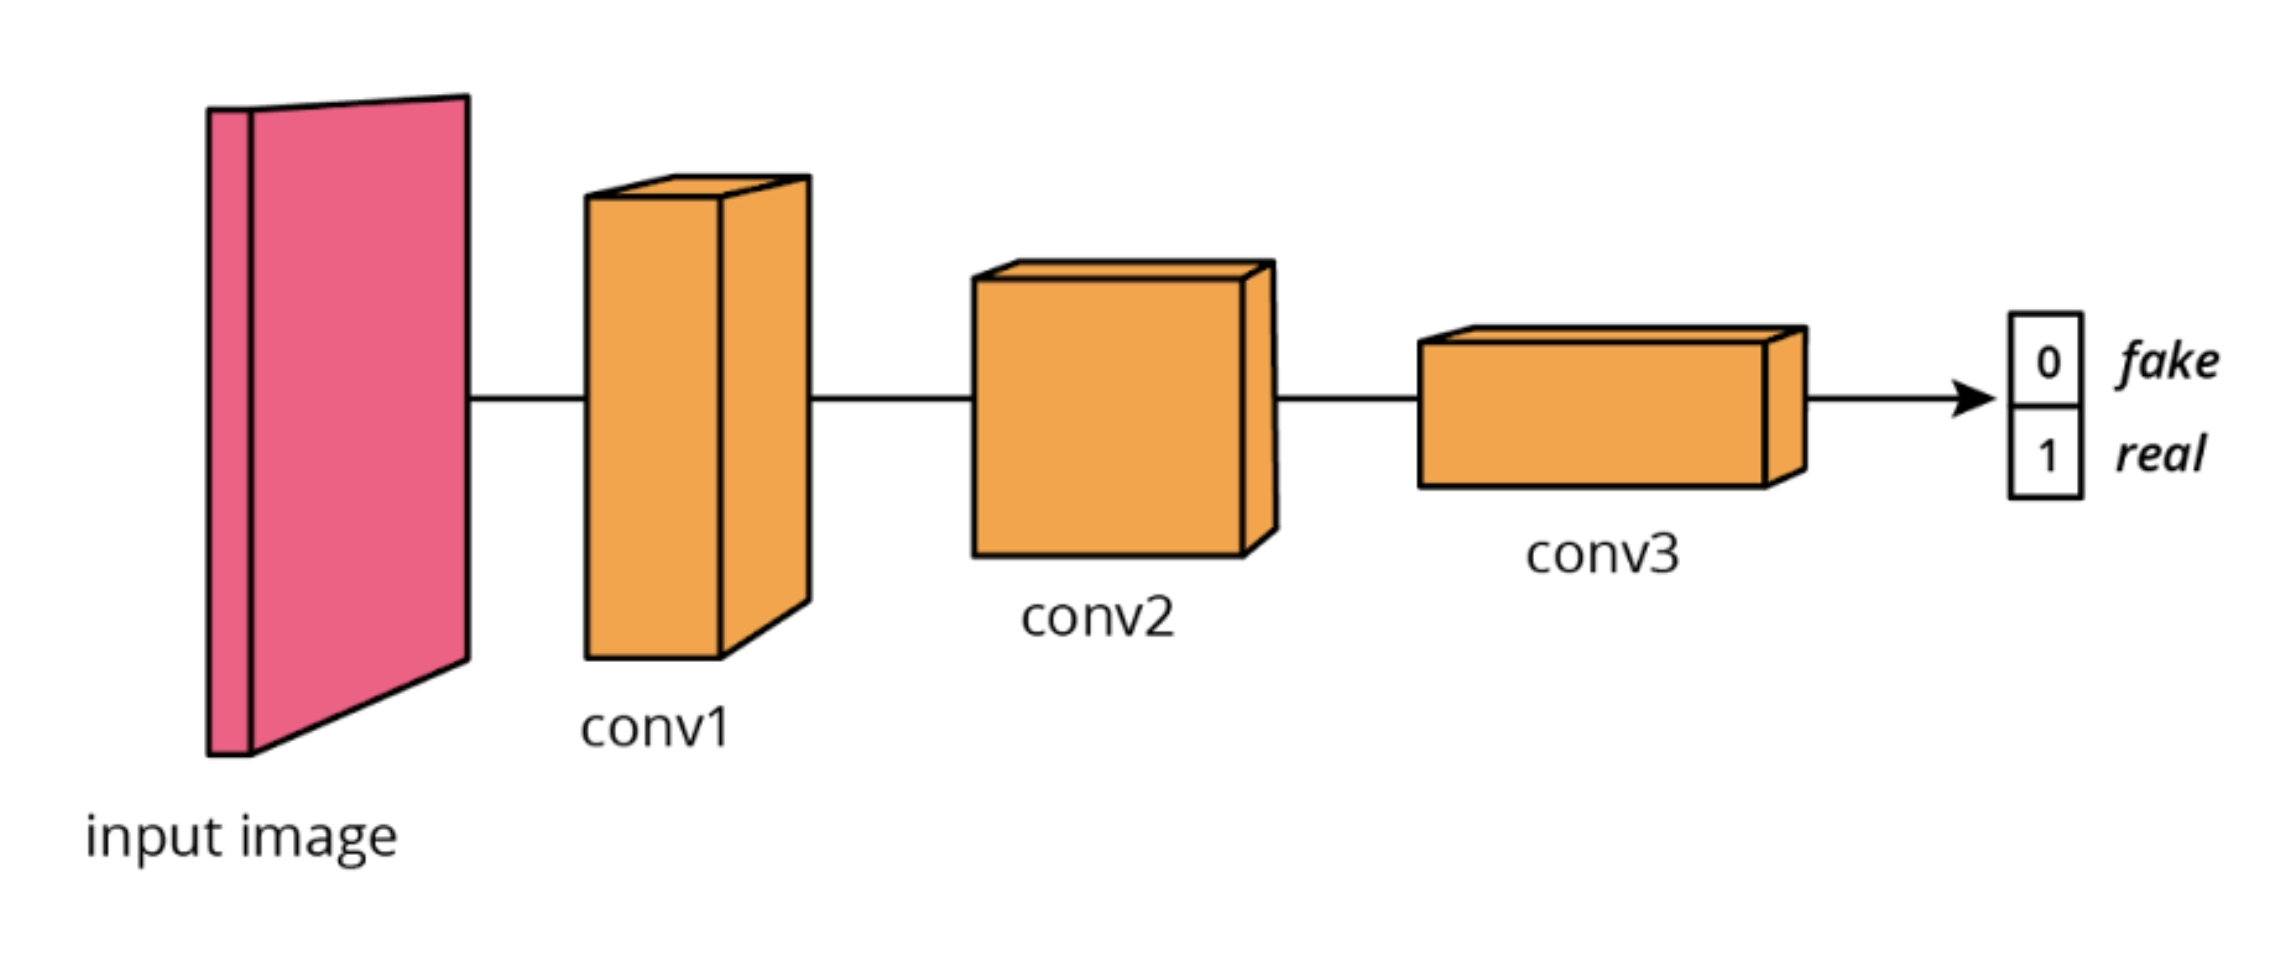
\includegraphics[width=1\linewidth]{img//genAdvNet//deepGAN/screen-shot-2022-05-10-at-9.21.49-am.jpeg}
\captionof{figure}{Big picture: GANs for complexity}

\section{Lesson Outline}
\href{https://www.youtube.com/watch?v=ADv_s4yanOU}{Youtube} \newline

In this lesson on \textbf{Deep Convolutional GANs} \textbf{(DCGANs)} we will cover the following topics:

\begin{itemize}
    \item Build DCGAN Discriminator and Generator
    \item Train a DCGAN Model
    \item Evaluate GANs using New Metrics
\end{itemize}

\section{Deep Convolutional GANs}
Youtube \newline

\textbf{Disclaimer:} This video mentions the Street View House Numbers Dataset or SVHN; however, you will actually be training a DCGAN model on the \href{https://www.cs.toronto.edu/~kriz/cifar.html}{\textbf{CIFAR10 dataset}}. Both datasets have a similar spatial resolution.

\subsection{Understanding a DCGAN}
In this lesson, you will be training a GAN on the \href{https://www.cs.toronto.edu/~kriz/cifar.html}{\textbf{CIFAR10 dataset,}} a labeled subset of the\href{http://people.csail.mit.edu/torralba/tinyimages/}{\textbf{ 80 million tiny images dataset}}. \newline

To improve model performance, convolutional layers will be used to make a DCGAN.

\begin{itemize}
    \item \textbf{DCGANs have generator and discriminator networks}, but the networks are made of convolutional layers that are designed to work with spatial data
    \item The discriminator will be a \textbf{convolutional neural network (CNN)} that classifies images are real or fake
    \item The generator will be a \textbf{transpose CNN} that upsamples a latent vector z and generates realistic images that can fool the discriminator.
\end{itemize}

\section{DCGAN, Discriminator}
\href{https://www.youtube.com/watch?v=5qVHECEB6H0}{Youtube} \newline

The \textbf{DCGAN Discriminator} is:

\begin{itemize}
    \item A convolutional neural network (CNN) with one fully connected layer at the end
    \item There are no max-pooling layers in the network
    \item \textbf{Down-sampling} is accomplished using convolutional layers that have a stride equal to 2
    \item \textbf{Batch normalization and Leaky ReLU activations} are applied to the outputs of all hidden layers
    \item After a series of downsampling convolutional layers, the final layer is flattened and connected to a single sigmoid unit
    \item The sigmoid unit output has a range from 0 to 1, indicating if an image is "real" or "fake"
\end{itemize}

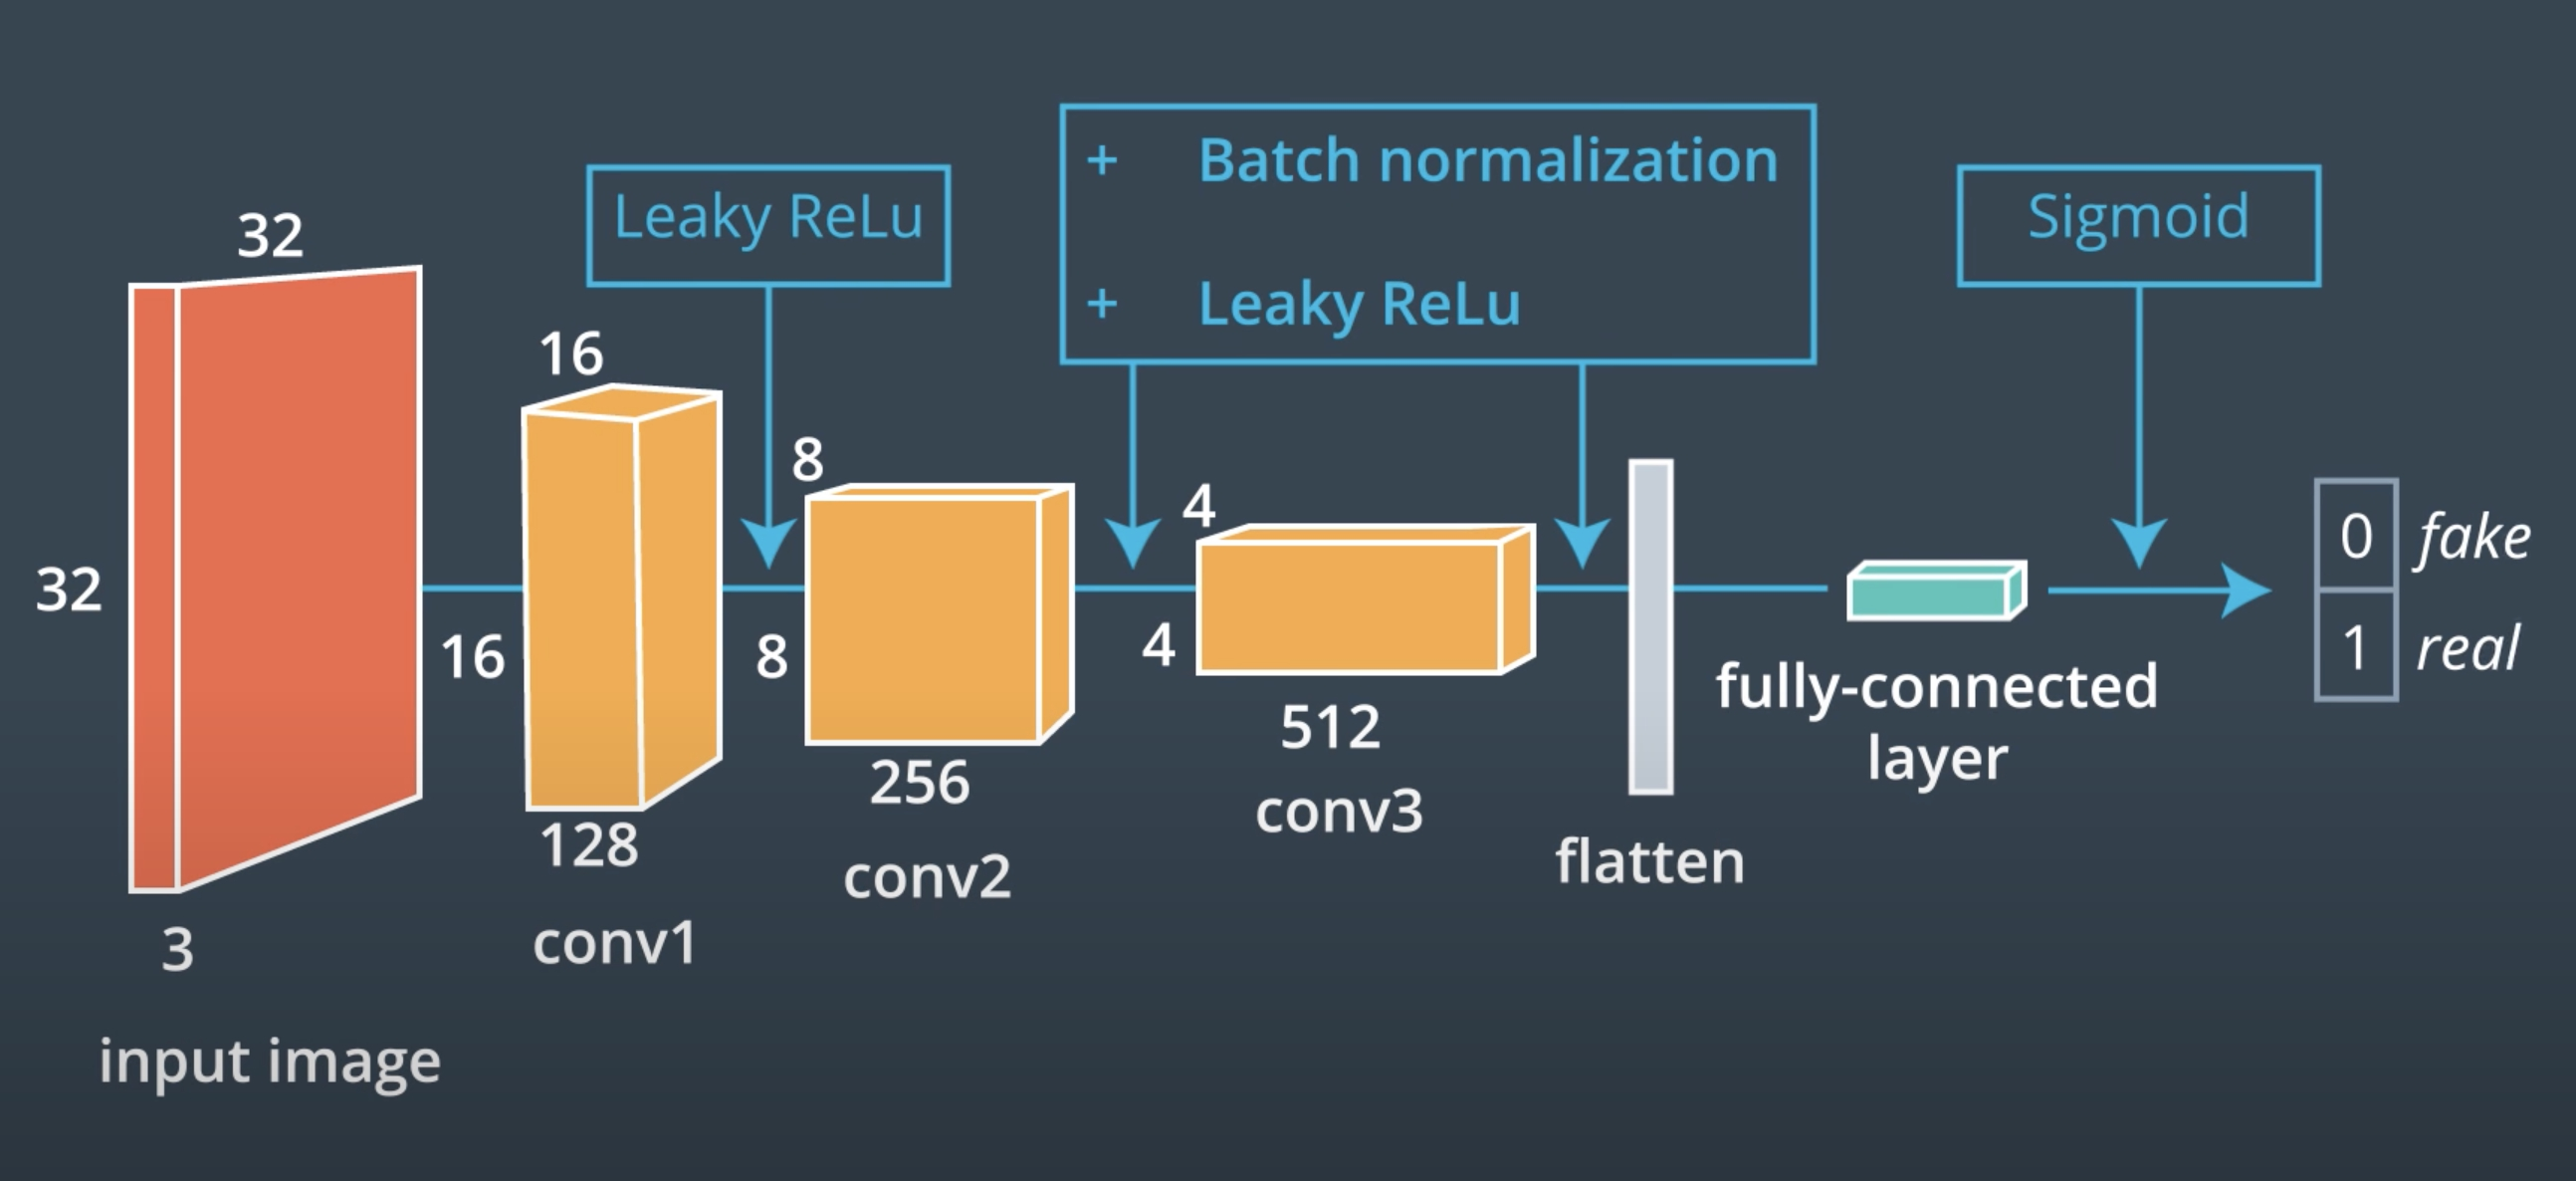
\includegraphics[width=1\linewidth]{img//genAdvNet//deepGAN/screen-shot-2022-05-10-at-10.27.10-am.jpeg}
\captionof{figure}{DCGAN Discriminator with convolutional layers progressively down-sampling}

\textbf{Leaky ReLu} – a function that will reduce any negative values by multiplying those values by some small coefficient, known as the \textbf{negative slope.}

\textbf{Batch Normalization} – scales the layer outputs to have a mean of 0 and variance of 1, to help the network train faster and reduce problems due to poor parameter initialization.

\subsection{DCGAN Paper}
It's always good to take a look at the original paper when you can. Many papers discuss both the theory and training details of deep learning networks, and you can read the DCGAN paper, \href{https://arxiv.org/pdf/1511.06434.pdf}{\textbf{Unsupervised Representational Learning with Deep Convolutional Generative Adversarial Networks}}.

\subsection{Quiz Question}
Which statements are true about the DCGAN discriminator?
\begin{itemize}
    \item \textbf{It uses Leaky ReLU activation instead of ReLU}
    \item \textbf{It uses convolution layer to decrease the input spatial resolution.}
    \item It also uses pooling layers to decrease the input spatial resolution.
\end{itemize}


\section{DCGAN Generator}
\href{https://www.youtube.com/watch?v=L_YXK_UPDmc}{Youtube} \newline

The task of a \textbf{DCGAN Generator} is to understand patterns in the underlying structure and features of the training data, in ways that allow it to create realistic generated images. \newline

The \textbf{DCGAN Generator}:

\begin{itemize}
    \item Has an input, random vector z
    \item Has an image output that can be sent to the discriminator
    \item Up-samples the vector z until it is the same shape as the training images
    \item Uses transposed convolutions
    \item ReLU activations and batch normalization is used on all hidden layers
    \item A tanh activation function is applied the the outputs of the final layer
\end{itemize}

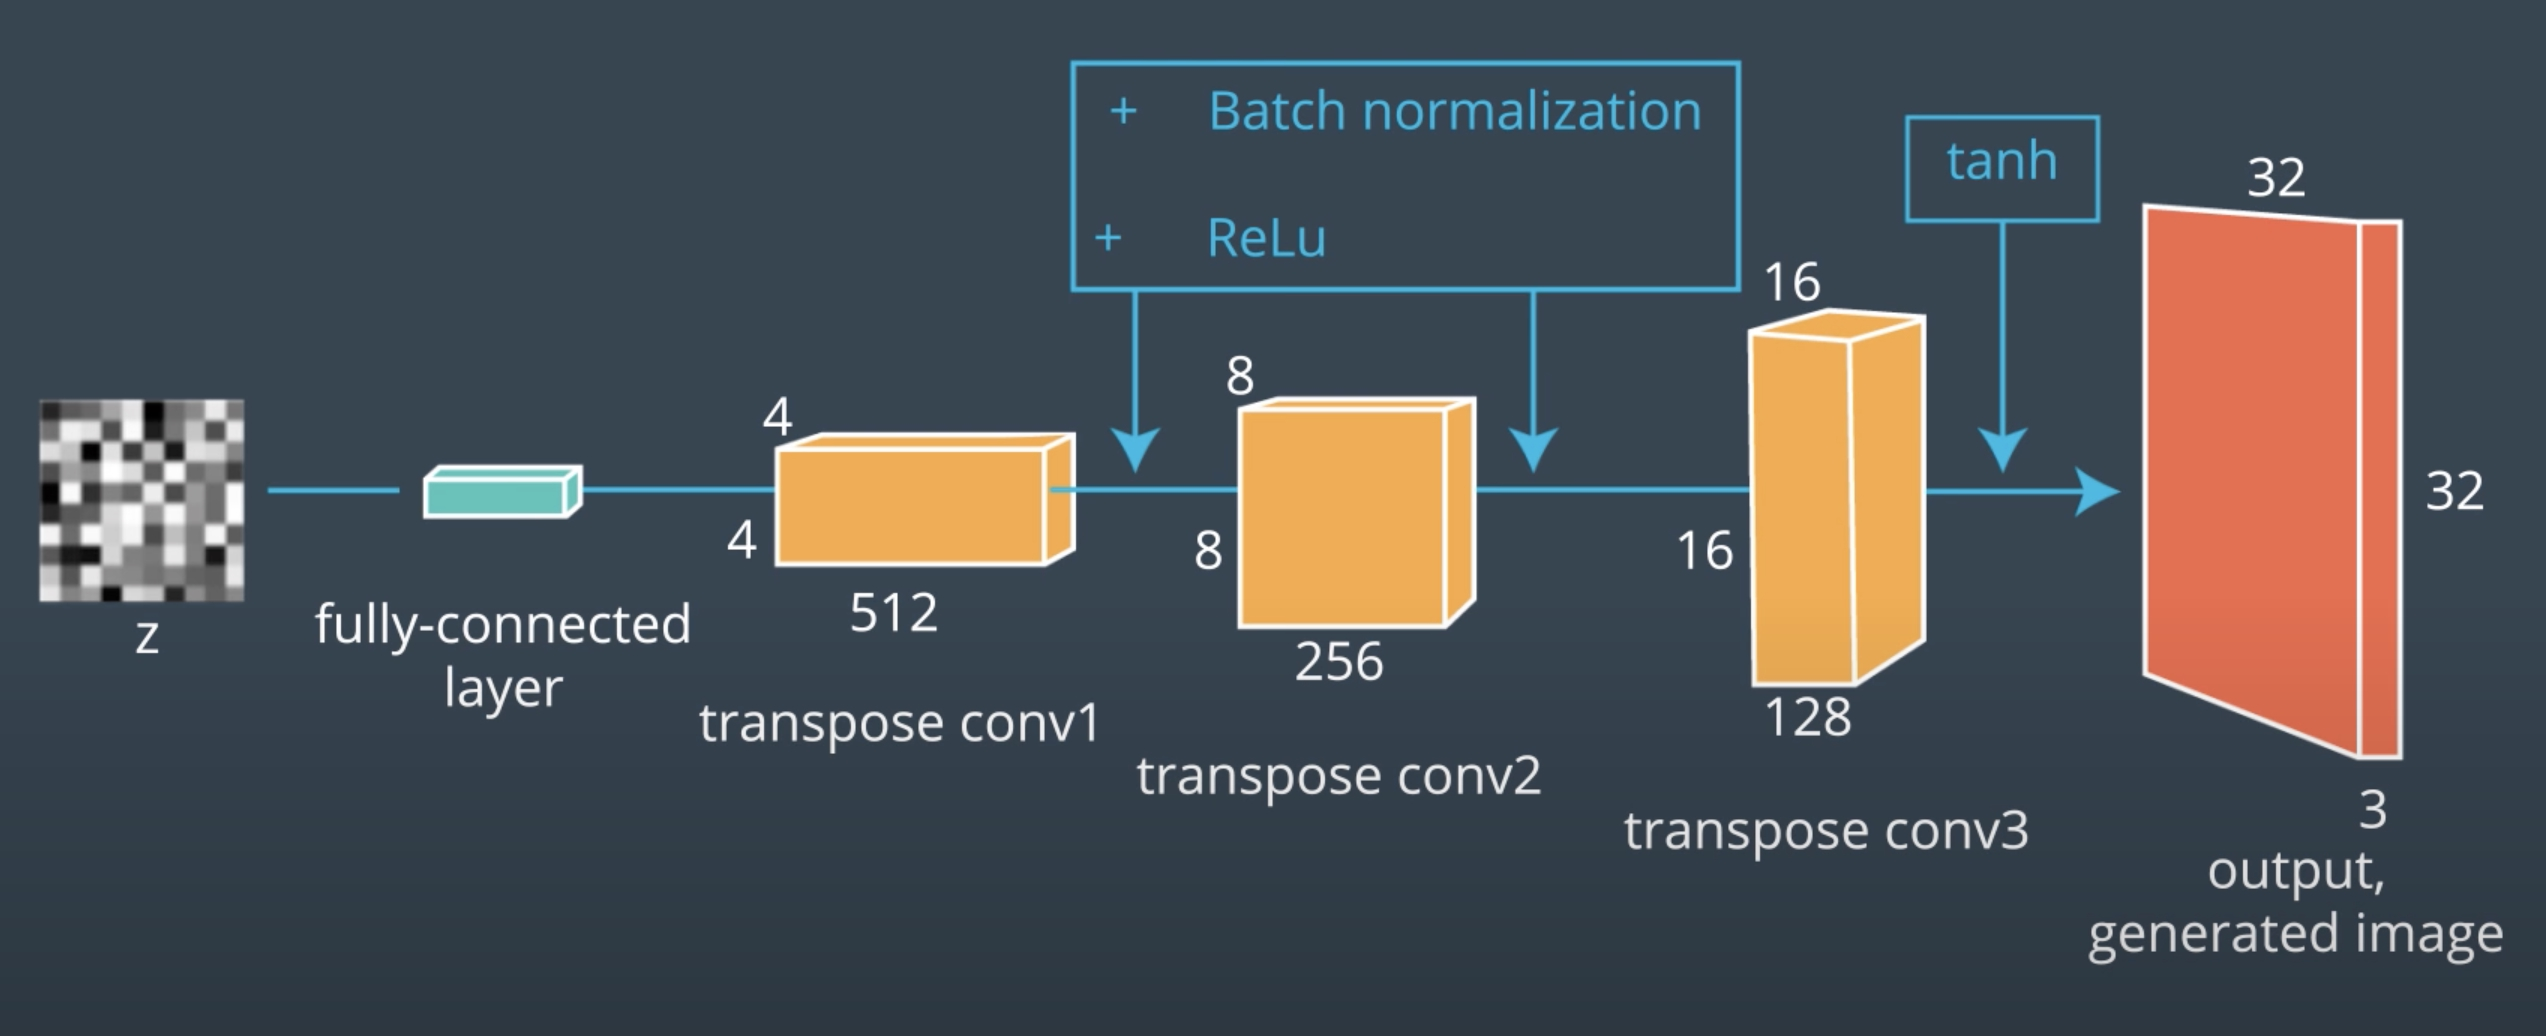
\includegraphics[width=1\linewidth]{img//genAdvNet//deepGAN/screen-shot-2022-05-10-at-10.26.17-am.jpeg}
\captionof{figure}{DCGAN Generator with transposed convolutions progressively up-sampling the layers}


\subsection{Generating Images}

To generate an image, the generator:

\begin{enumerate}
    \item Connects the input vector z to a fully connected layer
    \item The fully connected layer is reshaped to a 4x4 XY shape of a given depth
    \item A stack of larger layers is built by upsampling with transpose convolution
    \item Each layer is doubled in XY size using strides of 2, and depth is reduced
    \item The final output is a generated image the same size as the training images
\end{enumerate}

\subsection{Quiz Question}

Which statements are true about the DCGAN generator?
\begin{itemize}
    \item It only uses fully connected layers.
    \item \textbf{It outputs an RGB image in the -1 / 1 range.}
    \item \textbf{It uses transpose convolution layer to progressively increase the resolution.}
    \item It uses Leaky ReLU activation instead of ReLU.
\end{itemize}

\section{What is Batch Normalization?}
Batch normalization was introduced in Sergey Ioffe's and Christian Szegedy's 2015 paper \href{https://arxiv.org/pdf/1502.03167.pdf}{\textbf{Batch Normalization: Accelerating Deep Network Training by Reducing Internal Covariate Shift}}. The idea is that, instead of just normalizing the inputs to the network, we normalize the inputs to every layer \textit{within} the network.

\subsection{Batch Normalization}

It's called "batch" normalization because, during \textbf{training}, we normalize each layer's inputs by using the \textit{mean} and \textit{standard deviation} (or variance) of the values in the current batch. These are sometimes called the \textbf{batch statistics}.

\begin{quote}
Specifically, batch normalization normalizes the output of a previous layer by \textbf{subtracting the batch mean and dividing by the batch standard deviation}.

\end{quote}

Why might this help? Well, we know that normalizing the inputs to a network helps the network learn and converge to a solution. However, a network is a series of layers, where the output of one layer becomes the input to another. That means we can think of any layer in a neural network as the \textit{first} layer of a smaller network.

\subsubsection{Normalization at Every Layer}
For example, imagine a 3 layer network.

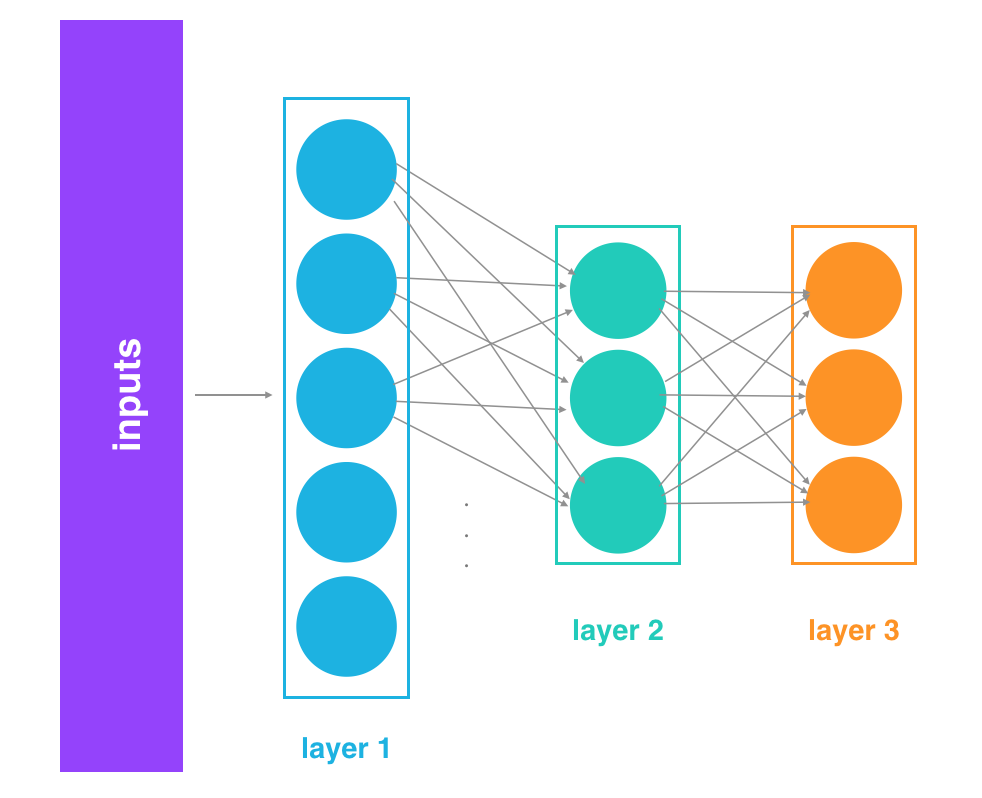
\includegraphics[width=0.5\linewidth]{img//genAdvNet//deepGAN/3-layers.png}
\captionof{figure}{Three layer network}

Instead of just thinking of it as a single network with inputs, layers, and outputs, think of the output of layer 1 as the input to a two layer network. This two layer network would consist of layers 2 and 3 in our original network.

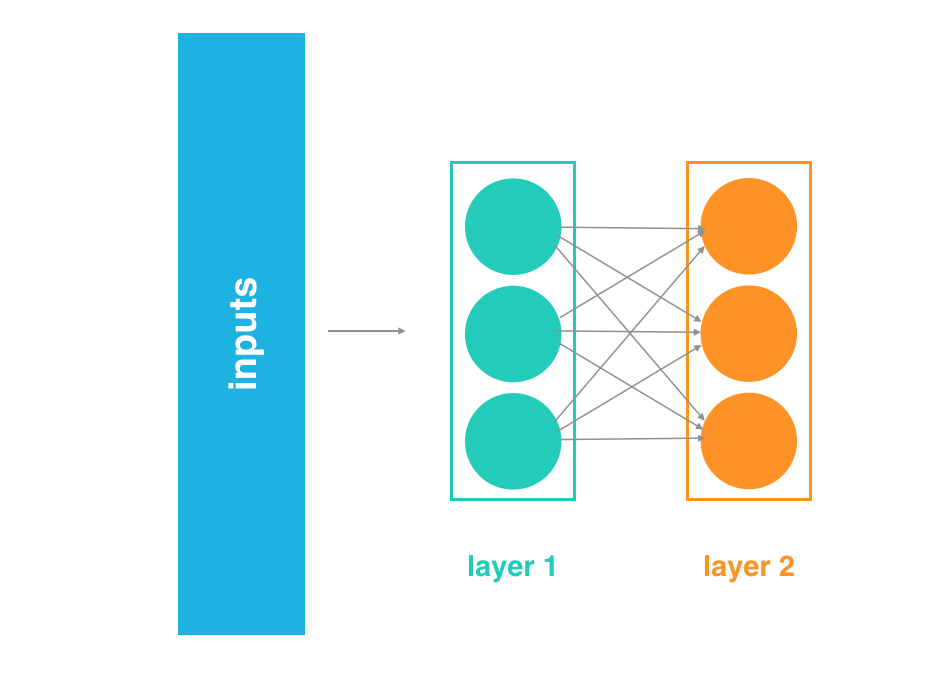
\includegraphics[width=0.5\linewidth]{img//genAdvNet//deepGAN/2-layers.png}
\captionof{figure}{Two layer network}

Likewise, the output of layer 2 can be thought of as the input to a single layer network, consisting only of layer 3.

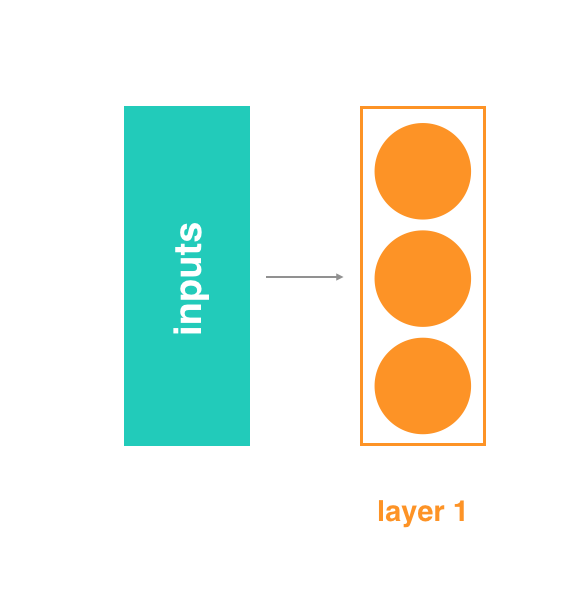
\includegraphics[width=0.5\linewidth]{img//genAdvNet//deepGAN/one-layer.png}
\captionof{figure}{One layer network}

When you think of it like this - as a series of neural networks feeding into each other - then it's easy to imagine how normalizing the inputs to each layer would help. It's just like normalizing the inputs to any other neural network, but you're doing it at \textbf{every layer (sub-network)}.

\subsubsection{Internal Covariate Shift}
Beyond the intuitive reasons, there are good mathematical reasons to motivate batch normalization. It helps combat what the authors call \textbf{internal covariate shift}.
\begin{quote}
In this case, internal covariate shift refers to the change in the distribution of the inputs to different layers. It turns out that training a network is most efficient when the distribution of inputs to each layer is similar!
\end{quote}
And batch normalization is one method of standardizing the distribution of layer inputs. This discussion is best handled \href{https://arxiv.org/pdf/1502.03167.pdf}{\textbf{the paper on Batch Normalization (ArXiv PDF)}} and in \href{http://www.deeplearningbook.org/}{\textbf{Deep Learning}}, a book you can read online written by Ian Goodfellow, Yoshua Bengio, and Aaron Courville. Specifically, check out the batch normalization section of \href{http://www.deeplearningbook.org/contents/optimization.html}{\textbf{Chapter 8: Optimization for Training Deep Models}}.

\subsection{The Math}
Next, let's do a deep dive into the math behind batch normalization. This is not critical for you to know, but it may help your understanding of this whole process!

\subsubsection{Getting the mean and variance}

In order to normalize the values, we first need to find the average value for the batch. If you look at the code, you can see that this is not the average value of the batch \textit{inputs}, but the average value coming \textit{out} of any particular layer before we pass it through its non-linear activation function and then feed it as an input to the \textit{next} layer.

We represent the average as \(\mu_B\) which is simply the sum of all of the values, \(x_i\) divided by the number of values,, \(m\): \[\mu_B = \frac{1}{m} \sum_{i=1}^m x_i\]
We then need to calculate the variance, or mean squared deviation, represented as \(\sigma_B^2\). If you aren't familiar with statistics, that simply means for each value \(x_i\), we subtract the average value (calculated earlier as \(mu_B\)), which gives us what's called the "deviation" for that value. We square the result to get the squared deviation. Sum up the results of doing that for each of the values, then divide by the number of values, again \(m\), to get the average, or mean, squared deviation. \[\sigma_B^2 = \frac{1}{m} \sum_{i=1}^m (x_i - \mu_B)^2\]
\subsubsection{Normalizing output values}
Once we have the mean and variance, we can use them to normalize the values with the following equation. For each value, it subtracts the mean and divides by the (almost) standard deviation. (You've probably heard of standard deviation many times, but if you have not studied statistics you might not know that the standard deviation is actually the square root of the mean squared deviation.) \[\hat{x}_i = \frac{x_i = \mu_B}{\sqrt{\sigma_B^2 + \epsilon}}\]
Above, we said "(almost) standard deviation". That's because the real standard deviation for the batch is calculated by \(\sqrt{\sigma_B^2}\), but the above formula adds the term epsilon before taking the square root. The epsilon can be any small, positive constant, ex. the value 0.001. It is there partially to make sure we don't try to divide by zero, but it also acts to increase the variance slightly for each batch. \newline

Why add this extra value and mimic an increase in variance? Statistically, this makes sense because even though we are normalizing one batch at a time, we are also trying to estimate the population distribution – the total training set, which itself an estimate of the larger population of inputs your network wants to handle. The variance of a population is \textit{typically} higher than the variance for any sample taken from that population, especially when you use a small sample size (a small sample is more likely to include values near the peak of a population distribution), so increasing the variance a little bit for each batch helps take that into account. \newline

At this point, we have a normalized value, represented as \(\hat{x}_i\). But rather than use it directly, we multiply it by a \textbf{gamma} value, and then add a \textbf{beta} value. Both gamma and beta are learnable parameters of the network and serve to scale and shift the normalized value, respectively. Because they are learnable just like weights, they give your network some extra knobs to tweak during training to help it learn the function it is trying to approximate. \[y_i = \gamma \hat{x}_i + \beta\]
We now have the final batch-normalized output of our layer, which we would then pass to a non-linear activation function like sigmoid, tanh, ReLU, Leaky ReLU, etc. In the original batch normalization paper, they mention that there might be cases when you'd want to perform the batch normalization \textit{after} the non-linearity instead of before, but it is difficult to find any uses like that in practice. \newline

\textbf{Next, take a look at the effect of batch normalization, by applying it to a PyTorch model!}

\section{Exercise Part 1: DCGAN Generator Discriminator}
In this notebook, you'll build a GAN using convolutional layers in the
generator and discriminator. This is called a Deep Convolutional GAN, or
DCGAN for short. The DCGAN architecture was first explored in 2016 and
has seen impressive results in generating new images; you can read the
\href{https://arxiv.org/pdf/1511.06434.pdf}{original paper, here}. \newline

You'll be training DCGAN on the
\href{https://www.cs.toronto.edu/~kriz/cifar.html}{CIFAR10} dataset.
These are color images of different classes, such as airplanes, dogs or
trucks. This dataset is much more complex and diverse than the MNIST
dataset and justifies the use of the DCGAN architecture.

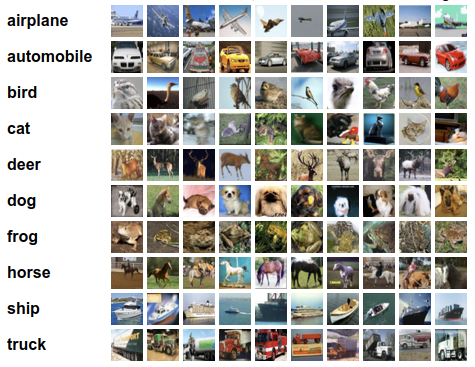
\includegraphics[width=1\linewidth]{img//genAdvNet//deepGAN/cifar10_data.png}

So, our goal is to create a DCGAN that can generate new,
realistic-looking images. We'll go through the following steps to do
this: 
\begin{itemize}
    \item Load in and pre-process the CIFAR10 dataset
    \item \textbf{Define discriminator and generator networks}
    \item Train these adversarial networks
    \item Visualize the loss over time and some sample, generated images
\end{itemize}

In this notebook, we will focus on defining the networks.

\paragraph{Deeper Convolutional Networks}

Since this dataset is more complex than our MNIST data, we'll need a
deeper network to accurately identify patterns in these images and be
able to generate new ones. Specifically, we'll use a series of
convolutional or transpose convolutional layers in the discriminator and
generator. It's also necessary to use batch normalization to get these
convolutional networks to train.\newline

Besides these changes in network structure, training the discriminator
and generator networks should be the same as before. That is, the
discriminator will alternate training on real and fake (generated)
images, and the generator will aim to trick the discriminator into
thinking that its generated images are real!

\subsection{Discriminator}

Here you'll build the discriminator. This is a convolutional classifier
like you've built before, only without any maxpooling layers. 
\begin{itemize}
    \item The inputs to the discriminator are 32x32x3 tensor images
    \item You'll want a few convolutional, hidden layers
    \item Then a fully connected layer for the output; as before, we want a sigmoid output, but we'll add that in the loss function, \href{https://pytorch.org/docs/stable/nn.html\#bcewithlogitsloss}{BCEWithLogitsLoss}, later
\end{itemize}

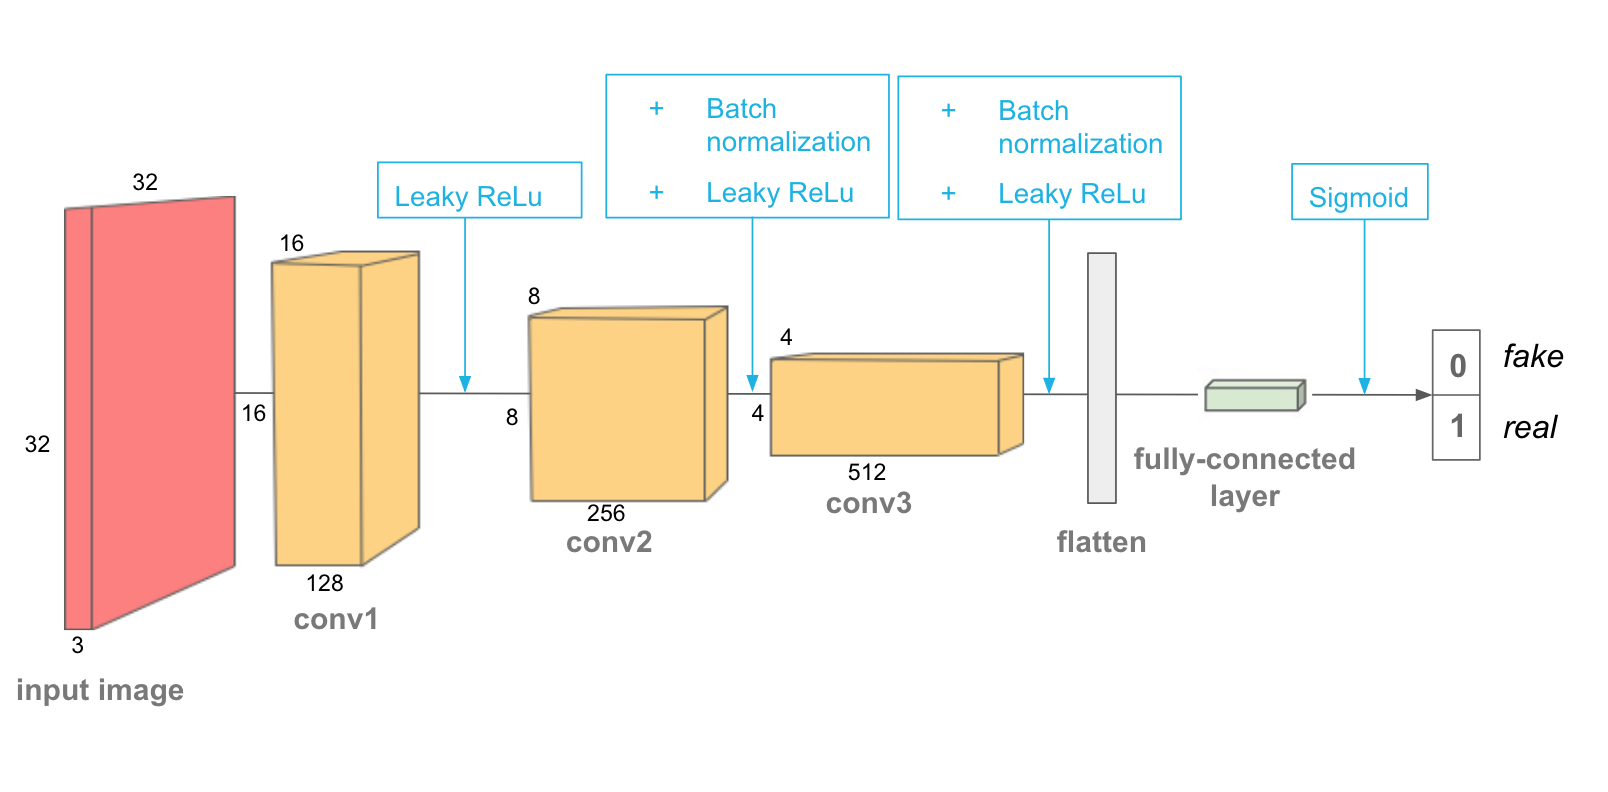
\includegraphics[width=1\linewidth]{img//genAdvNet//deepGAN/conv_discriminator.png}

For the depths of the convolutional layers I suggest starting with 32
filters in the first layer, then double that depth as you add layers (to
64, 128, etc.). Note that in the DCGAN paper, they did all the
downsampling using only strided convolutional layers with no maxpooling
layers. \newline

You'll also want to use batch normalization with
\href{https://pytorch.org/docs/stable/nn.html\#batchnorm2d}{nn.BatchNorm2d}
on each layer \textbf{except} the first convolutional layer and final,
linear output layer.

\paragraph{\texorpdfstring{Helper \texttt{ConvBlock}
module}{Helper ConvBlock module}}

In general, each layer should look something like convolution
\textgreater{} batch norm \textgreater{} leaky ReLU, and so we'll define
a \textbf{custom torch Module} to put these layers together. This module
will create a sequential series of a convolutional + an optional batch
norm layer.\newline

Note: It is also suggested that you use a \textbf{kernel\_size of 4} and
a \textbf{stride of 2} for strided convolutions.

\subsubsection{First exercise}

Implement the \lstinline{ConvBlock} module below and use
it for your implementation of the
\lstinline{Discriminator} module. Your discriminator
should take a 32x32x3 image as input and output a single logit.

\begin{lstlisting}[language=Python]
import torch
import torch.nn as nn

import tests
\end{lstlisting}

\begin{lstlisting}[language=Python]
class ConvBlock(nn.Module):
    """
    A convolutional block is made of 3 layers: Conv -> BatchNorm -> Activation.
    args:
    - in_channels: number of channels in the input to the conv layer
    - out_channels: number of filters in the conv layer
    - kernel_size: filter dimension of the conv layer
    - batch_norm: whether to use batch norm or not
    """
    def __init__(self, in_channels: int, out_channels: int, kernel_size: int, batch_norm: bool = True):
        super(ConvBlock, self).__init__()
        self.conv = nn.Conv2d(in_channels=in_channels, 
                              out_channels=out_channels, 
                              kernel_size=kernel_size, 
                              stride=2, 
                              padding=1,
                              bias=False)
        self.activation = nn.LeakyReLU(negative_slope=0.2)
        self.is_batch_norm = batch_norm
        self.bn = nn.BatchNorm2d(out_channels)
        
    def forward(self, x: torch.Tensor) -> torch.Tensor:
        x = self.conv(x)
        if self.is_batch_norm:
            x = self.bn(x)
        x = self.activation(x)
        return x
\end{lstlisting}

\begin{lstlisting}[language=Python]
class Discriminator(nn.Module):
    """
    The discriminator model adapted from the DCGAN paper. It should only contains a few layers.
    args:
    - conv_dim: control the number of filters
    """
    def __init__(self, conv_dim: int):
        super(Discriminator, self).__init__()
        self.conv_dim = conv_dim
        
        # input: 32x32, 1st layer no batch norm
        self.conv1 = ConvBlock(in_channels=3, 
                               out_channels=self.conv_dim, 
                               kernel_size=4, 
                               batch_norm = False)
        # input: 16x16
        self.conv2 = ConvBlock(in_channels=self.conv_dim, 
                               out_channels=self.conv_dim*2, 
                               kernel_size=4)
        # input: 8 x 8
        self.conv3 = ConvBlock(in_channels=self.conv_dim*2, 
                               out_channels=self.conv_dim*4, 
                               kernel_size=4)
        # output: 4x4
        
        # flatten
        self.flatten = nn.Flatten()
        # fully connected layer
        self.fcl = nn.Linear(conv_dim*4*4*4, 1) # self.conv_dimx4 (from the out channel) x 4 x 4
    def forward(self, x):
        x = self.conv1(x)
        x = self.conv2(x)
        x = self.conv3(x)
        x = self.flatten(x)
        x = self.fcl(x)  
        return x
\end{lstlisting}

\begin{lstlisting}[language=Python]
discriminator = Discriminator(64)
print(discriminator)
\end{lstlisting}

\begin{lstlisting}
Discriminator(
  (conv1): ConvBlock(
    (conv): Conv2d(3, 64, kernel_size=(4, 4), stride=(2, 2), padding=(1, 1), bias=False)
    (activation): LeakyReLU(negative_slope=0.2)
    (bn): BatchNorm2d(64, eps=1e-05, momentum=0.1, affine=True, track_running_stats=True)
  )
  (conv2): ConvBlock(
    (conv): Conv2d(64, 128, kernel_size=(4, 4), stride=(2, 2), padding=(1, 1), bias=False)
    (activation): LeakyReLU(negative_slope=0.2)
    (bn): BatchNorm2d(128, eps=1e-05, momentum=0.1, affine=True, track_running_stats=True)
  )
  (conv3): ConvBlock(
    (conv): Conv2d(128, 256, kernel_size=(4, 4), stride=(2, 2), padding=(1, 1), bias=False)
    (activation): LeakyReLU(negative_slope=0.2)
    (bn): BatchNorm2d(256, eps=1e-05, momentum=0.1, affine=True, track_running_stats=True)
  )
  (flatten): Flatten(start_dim=1, end_dim=-1)
  (fcl): Linear(in_features=4096, out_features=1, bias=True)
)
\end{lstlisting}

\begin{lstlisting}[language=Python]
tests.check_discriminator(discriminator)
\end{lstlisting}

\begin{lstlisting}
Congrats, you successfully implemented your discriminator
\end{lstlisting}

\subsection{Generator}

Next, you'll build the generator network. The input will be our noise
vector \lstinline{z}, as before. And, the output will be a
\(tanh\) output, but this time with size 32x32 which is the size of our
CIFAR10 images.

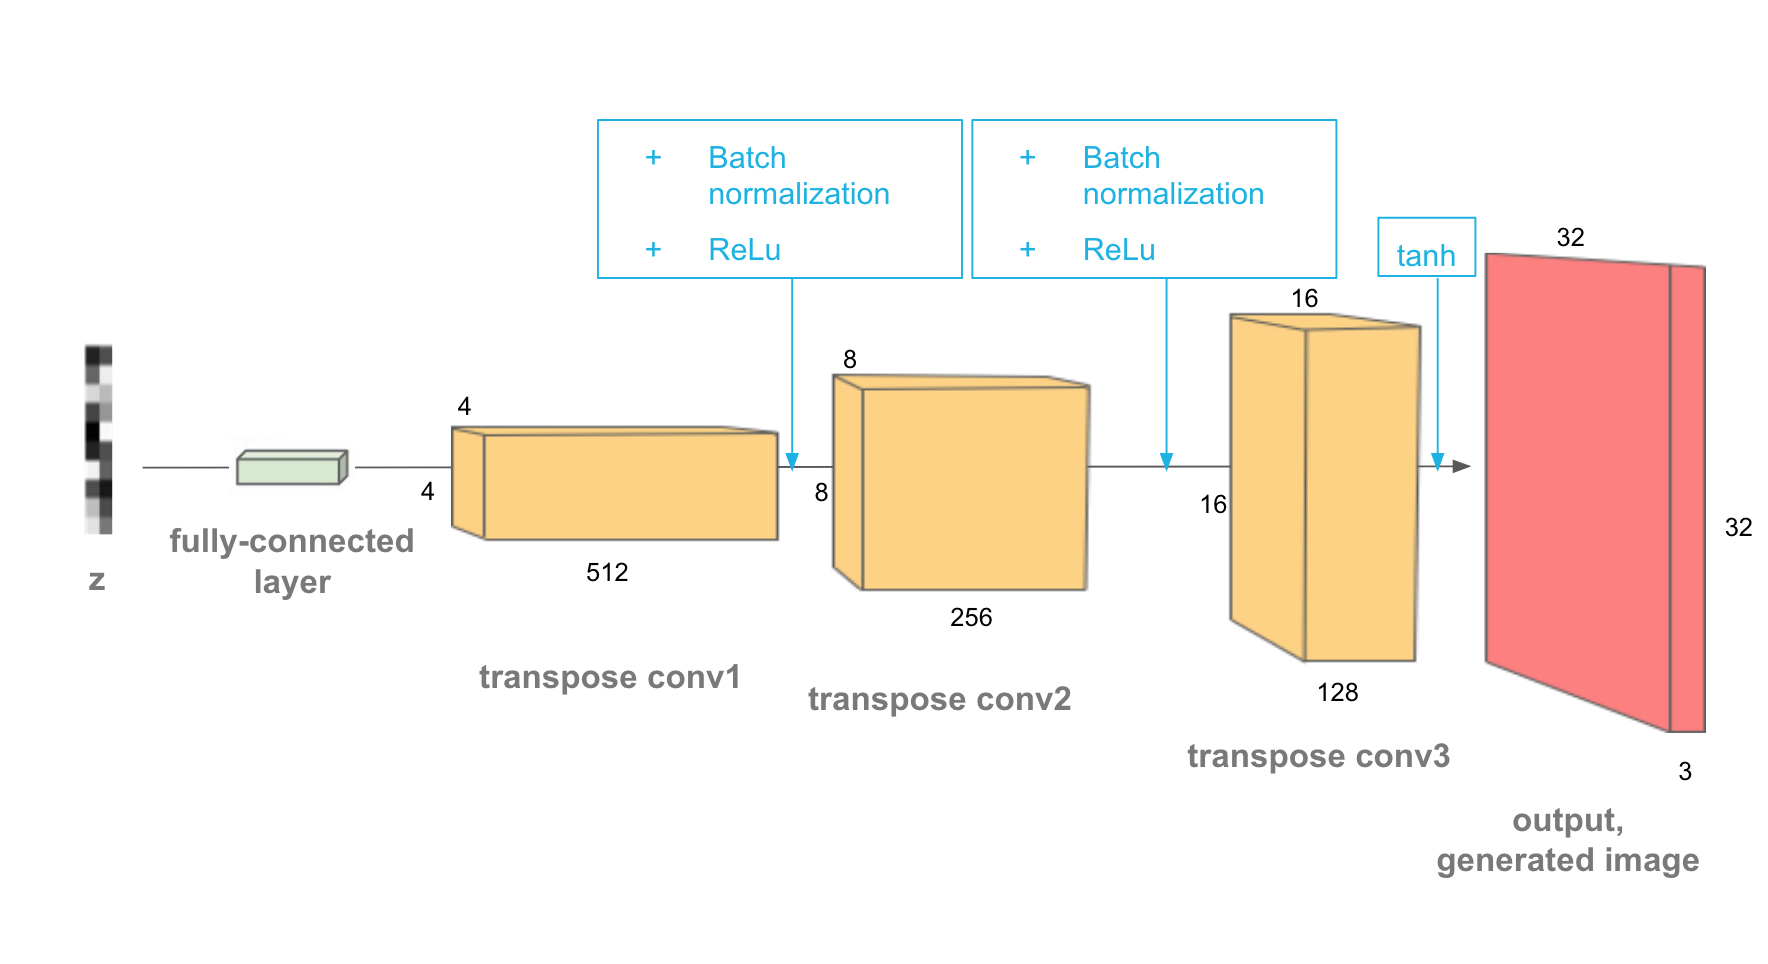
\includegraphics[width=1\linewidth]{img//genAdvNet//deepGAN/conv_generator.png}

What's new here is we'll use transpose convolutional layers to create
our new images. 
\begin{itemize}
    \item The first layer is a fully connected layer which is reshaped into a deep and narrow layer, something like 4x4x512.
    \item  Then, we use batch normalization and a leaky ReLU activation.
    \item Next is a series of \href{https://pytorch.org/docs/stable/nn.html\#convtranspose2d}{transpose convolutional layers}, where you typically halve the depth and double the width and height of the previous layer.
    \item And, we'll apply batch normalization and ReLU to all but the last of these hidden layers. Where we will just apply a \lstinline{tanh} activation.
\end{itemize}

\paragraph{\texorpdfstring{Helper \texttt{DeconvBlock}
module}{Helper DeconvBlock module}}

For each of these layers, the general scheme is transpose convolution
> batch norm > ReLU, and so we'll define a
function to put these layers together. This function will create a
sequential series of a transpose convolutional + an optional batch norm
layer. We'll create these using PyTorch's Sequential container, which
takes in a list of layers and creates layers according to the order that
they are passed in to the Sequential constructor.\newline

Note: It is also suggested that you use a \textbf{kernel\_size of 4} and
a \textbf{stride of 2} for transpose convolutions.

\paragraph{Second exercise}

Implement the \lstinline{DeconvBlock} module below and use
it for your implementation of the \lstinline{Generator}
module. Your generator should take a latent vector of dimension 128 as
input and output a 32x32x3 image.

\begin{lstlisting}[language=Python]
class DeconvBlock(nn.Module):
    """
    A "de-convolutional" block is made of 3 layers: ConvTranspose -> BatchNorm -> Activation.
    args:
    - in_channels: number of channels in the input to the conv layer
    - out_channels: number of filters in the conv layer
    - kernel_size: filter dimension of the conv layer
    - stride: stride of the conv layer
    - padding: padding of the conv layer
    - batch_norm: whether to use batch norm or not
    """
    def __init__(self, 
                 in_channels: int, 
                 out_channels: int, 
                 kernel_size: int, 
                 stride: int,
                 padding: int,
                 batch_norm: bool = True):
        super(DeconvBlock, self).__init__()
        self.tConv = nn.ConvTranspose2d(in_channels=in_channels,
                                         out_channels=out_channels, 
                                         kernel_size=kernel_size, 
                                         stride=stride, 
                                         padding=padding,
                                         bias=False)
        self.activation = nn.ReLU()
        self.bn = nn.BatchNorm2d(out_channels)
        self.batch_norm = batch_norm
        
    def forward(self, x: torch.Tensor) -> torch.Tensor:
        x = self.tConv(x)
        if self.batch_norm:
            x = self.bn(x)
        x = self.activation(x)
        return x
\end{lstlisting}

\begin{lstlisting}[language=Python]
class Generator(nn.Module):
    """
    The generator model adapted from DCGAN
    args:
    - latent_dim: dimension of the latent vector
    - conv_dim: control the number of filters in the convtranspose layers
    """
    def __init__(self, latent_dim: int, conv_dim: int = 32):
        super(Generator, self).__init__()
        self.latent_dim = latent_dim
        self.conv_dim = conv_dim
        self.layer1 = DeconvBlock(in_channels=self.latent_dim, 
                                  out_channels=self.conv_dim*4, 
                                  kernel_size=4, 
                                  stride=1, 
                                  padding=0)
        self.layer2 = DeconvBlock(in_channels=self.conv_dim*4, 
                                  out_channels=self.conv_dim*2, 
                                  kernel_size=4, 
                                  stride=2, 
                                  padding=1)
        self.layer3 = DeconvBlock(in_channels=self.conv_dim*2, 
                                  out_channels=self.conv_dim, 
                                  kernel_size=4, 
                                  stride=2, 
                                  padding=1)
        self.layer4 = nn.ConvTranspose2d(in_channels=self.conv_dim,
                                         out_channels=3, 
                                         kernel_size=4, 
                                         stride=2, 
                                         padding=1)
        self.last_activation = nn.Tanh()
        
    def forward(self, x):
        x = self.layer1(x)
        x = self.layer2(x)
        x = self.layer3(x)
        x = self.layer4(x)
        x = self.last_activation(x)
        return x
\end{lstlisting}

\begin{lstlisting}[language=Python]
generator = Generator(128)
print(generator)
\end{lstlisting}

\begin{lstlisting}
Generator(
  (layer1): DeconvBlock(
    (tConv): ConvTranspose2d(128, 128, kernel_size=(4, 4), stride=(1, 1), bias=False)
    (activation): ReLU()
    (bn): BatchNorm2d(128, eps=1e-05, momentum=0.1, affine=True, track_running_stats=True)
  )
  (layer2): DeconvBlock(
    (tConv): ConvTranspose2d(128, 64, kernel_size=(4, 4), stride=(2, 2), padding=(1, 1), bias=False)
    (activation): ReLU()
    (bn): BatchNorm2d(64, eps=1e-05, momentum=0.1, affine=True, track_running_stats=True)
  )
  (layer3): DeconvBlock(
    (tConv): ConvTranspose2d(64, 32, kernel_size=(4, 4), stride=(2, 2), padding=(1, 1), bias=False)
    (activation): ReLU()
    (bn): BatchNorm2d(32, eps=1e-05, momentum=0.1, affine=True, track_running_stats=True)
  )
  (layer4): ConvTranspose2d(32, 3, kernel_size=(4, 4), stride=(2, 2), padding=(1, 1), bias=False)
  (last_activation): Tanh()
)
\end{lstlisting}

\begin{lstlisting}[language=Python]
tests.check_generator(generator, 128)
\end{lstlisting}

\begin{lstlisting}
Congrats, you successfully implemented your discriminator
\end{lstlisting}


Solution on \href{https://www.youtube.com/watch?v=VSjGD3VtsZU}{Youtube}

\subsection{Why no bias?}

The reason there is no \verb|bias| for our convolutional layers is because we have batch normalization applied to their outputs. The goal of batch normalization is to get outputs with:

\begin{itemize}
    \item mean = 0
    \item standard deviation = 1
\end{itemize}
Since we want the mean to be 0, we do \textit{not} want to add an offset (bias) that will deviate from 0. We want the outputs of our convolutional layer to rely only on the coefficient weights. \newline

This exercise solution is contained within the exercise notebook. Simply click the Jupyter icon to access the solution file.

\section{Benefits of Batch Normalization}

\subsection{Adding Batch Normalization Layers to a PyTorch Model}
In the last notebook, you saw how a model with batch normalization applied reached a lower training loss and higher test accuracy! There are quite a few comments in that code, and I just want to recap a few of the most important lines. \newline

To add batch normalization layers to a PyTorch model:

\begin{itemize}
    \item You add batch normalization to layers inside the\lstinline{__init__} function.
    \item Layers with batch normalization do not include a bias term. So, for linear or convolutional layers, you'll need to set \lstinline{bias=False} if you plan to add batch normalization on the outputs.
    \item You can use PyTorch's \href{https://pytorch.org/docs/stable/generated/torch.nn.BatchNorm1d.html}{\textbf{BatchNorm1d}} function to handle the math on linear outputs \textit{or} \href{https://pytorch.org/docs/stable/generated/torch.nn.BatchNorm2d.html}{\textbf{BatchNorm2d}} for 2D outputs, like filtered images from convolutional layers.
    \item You add the batch normalization layer \textit{before} calling the activation function, so it always goes layer > batch norm > activation.
\end{itemize}
Finally, when you tested your model, you set it to \lstinline{.eval()} mode, which ensures that the batch normalization layers use the \textit{population}rather than the \textit{batch} mean and variance (as they do during training).

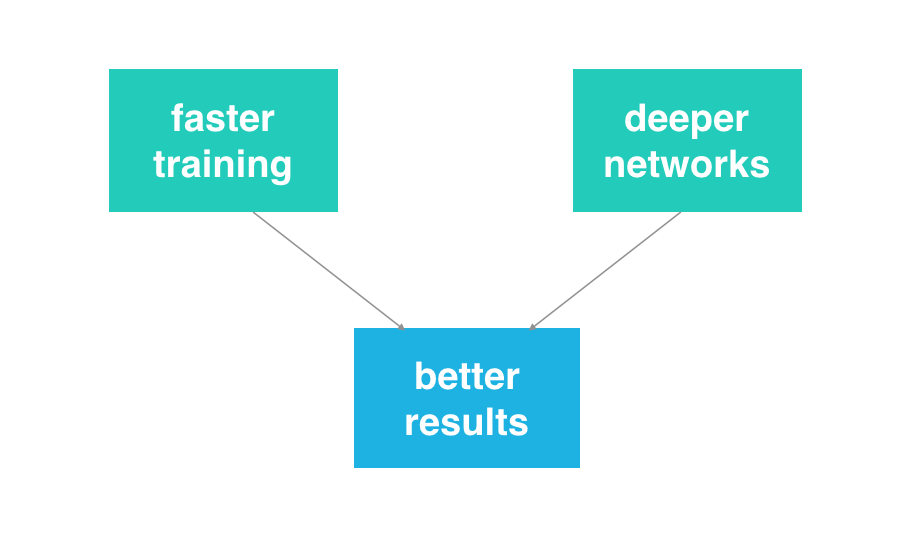
\includegraphics[width=0.5\linewidth]{img//genAdvNet//deepGAN/screen-shot-2018-11-07-at-4.53.24-pm.png}
\captionof{figure}{Benefits of batch normalization}

\subsubsection{The takeaway}
By using batch normalization to normalize the inputs at each layer of a network, we can make these inputs more consistent and thus reduce oscillations that may happen in gradient descent calculations. This helps us build deeper models that also converge faster!
\begin{quote}
Take a look at the \href{https://pytorch.org/docs/stable/nn.html\#batchnorm2d}{\textbf{PyTorch BatchNorm2d documentation}} to learn more about how to add batch normalization to a model, and how data is transformed during training (and evaluation).

\end{quote}
\subsection{Benefits of Batch Normalization}
Batch normalization optimizes network training. It has been shown to have several benefits:
\begin{enumerate}
    \item \textbf{Networks train faster} – Each training \textit{iteration} will actually be slower because of the extra calculations during the forward pass and the additional hyperparameters to train during back propagation. However, it should converge much more quickly, so training should be faster overall.
    \item \textbf{Allows higher learning rates} – Gradient descent usually requires small learning rates for the network to converge. And as networks get deeper, their gradients get smaller during back propagation so they require even more iterations. Using batch normalization allows us to use much higher learning rates, which further increases the speed at which networks train.
    \item \textbf{Makes weights easier to initialize} – Weight initialization can be difficult, and it's even more difficult when creating deeper networks. Batch normalization seems to allow us to be much less careful about choosing our initial starting weights.
    \item \textbf{Makes more activation functions viable} – Some activation functions do not work well in some situations. Sigmoids lose their gradient pretty quickly, which means they can't be used in deep networks. And ReLUs often die out during training, where they stop learning completely, so we need to be careful about the range of values fed into them. Because batch normalization regulates the values going into each activation function, non-linearlities that don't seem to work well in deep networks actually become viable again.
    \item \textbf{Simplifies the creation of deeper networks} – Because of the first 4 items listed above, it is easier to build and faster to train deeper neural networks when using batch normalization. And it's been shown that deeper networks generally produce better results, so that's great.
    \item \textbf{Provides a bit of regularization} – Batch normalization adds a little noise to your network. In some cases, such as in Inception modules, batch normalization has been shown to work as well as dropout. But in general, consider batch normalization as a bit of extra regularization, possibly allowing you to reduce some of the dropout you might add to a network.
    \item \textbf{May give better results overall} – Some tests seem to show batch normalization actually improves the training results. However, it's really an optimization to help train faster, so you shouldn't think of it as a way to make your network better. But since it lets you train networks faster, that means you can iterate over more designs more quickly. It also lets you build deeper networks, which are usually better. So when you factor in everything, you're probably going to end up with better results if you build your networks with batch normalization.
\end{enumerate}

\section{Optimization Strategy / Hyperparameters}
\href{https://www.youtube.com/watch?v=0Im7Nfs2o4k&t=1s}{Youtube} \newline

\begin{itemize}
    \item Training GANs is hard. Often it is an optimization issue.
    \item Regularize the discriminator, e.g. drop out layers, label smoothing, noisy labels (flip labels during the discriminator update)
    \item GANs are sensitive to hyperparameters. Experiment with hyperparameters
    \begin{itemize}
        \item Most value gained from the learning rate and optimizer
    \end{itemize}
    \item Average Discriminator and Generator during training using an exponential moving average
\end{itemize}
\subsubsection{Two Times Update Rule [TTUR]}
Another approach for better GAN convergence consists in using the \href{https://arxiv.org/pdf/1706.08500.pdf}{\textbf{Two Times Update Rule (TTUR)}}. This approach consists in running more update steps for the discriminator than for the generator. For example, for each update of the generator, we run 3 updates of the discriminator.\newline

Another way is to have a slightly higher learning rate for the discriminator. An example of TTUR can be found in the \href{https://github.com/bioinf-jku/TTUR/blob/master/WGAN_GP/gan_64x64_FID.py\#L44}{\textbf{official implementation by the Institute of Bioinformatics, Johannes Kepler University Linz}}.

\subsubsection{\href{http://karpathy.github.io/2019/04/25/recipe/}{\textbf{A recipe for training Neural Networks}}}

The above link is a \textbf{great} resource to use when debugging neural networks. It applies to any type of deep learning model, including GAN and was written by Andrej Karpathy, the head of AI at Tesla. Definitely a recommended read!

\subsection{Question 1 of 2}
Why is training GAN hard? (Check all correct choices)
\begin{itemize}
    \item \textbf{The discriminator's job is much easier and it can easily overcome the generator.}
    \item \textbf{GANs are harder to monitor because fluctuating losses are not a sign that the sign is going poorly.}
    \item \textbf{The minimax game is inherently hard because the equilibrium between generator and discriminator requires solving a hard optimization problem.}
\end{itemize}


\subsection{Question 2 of 2}

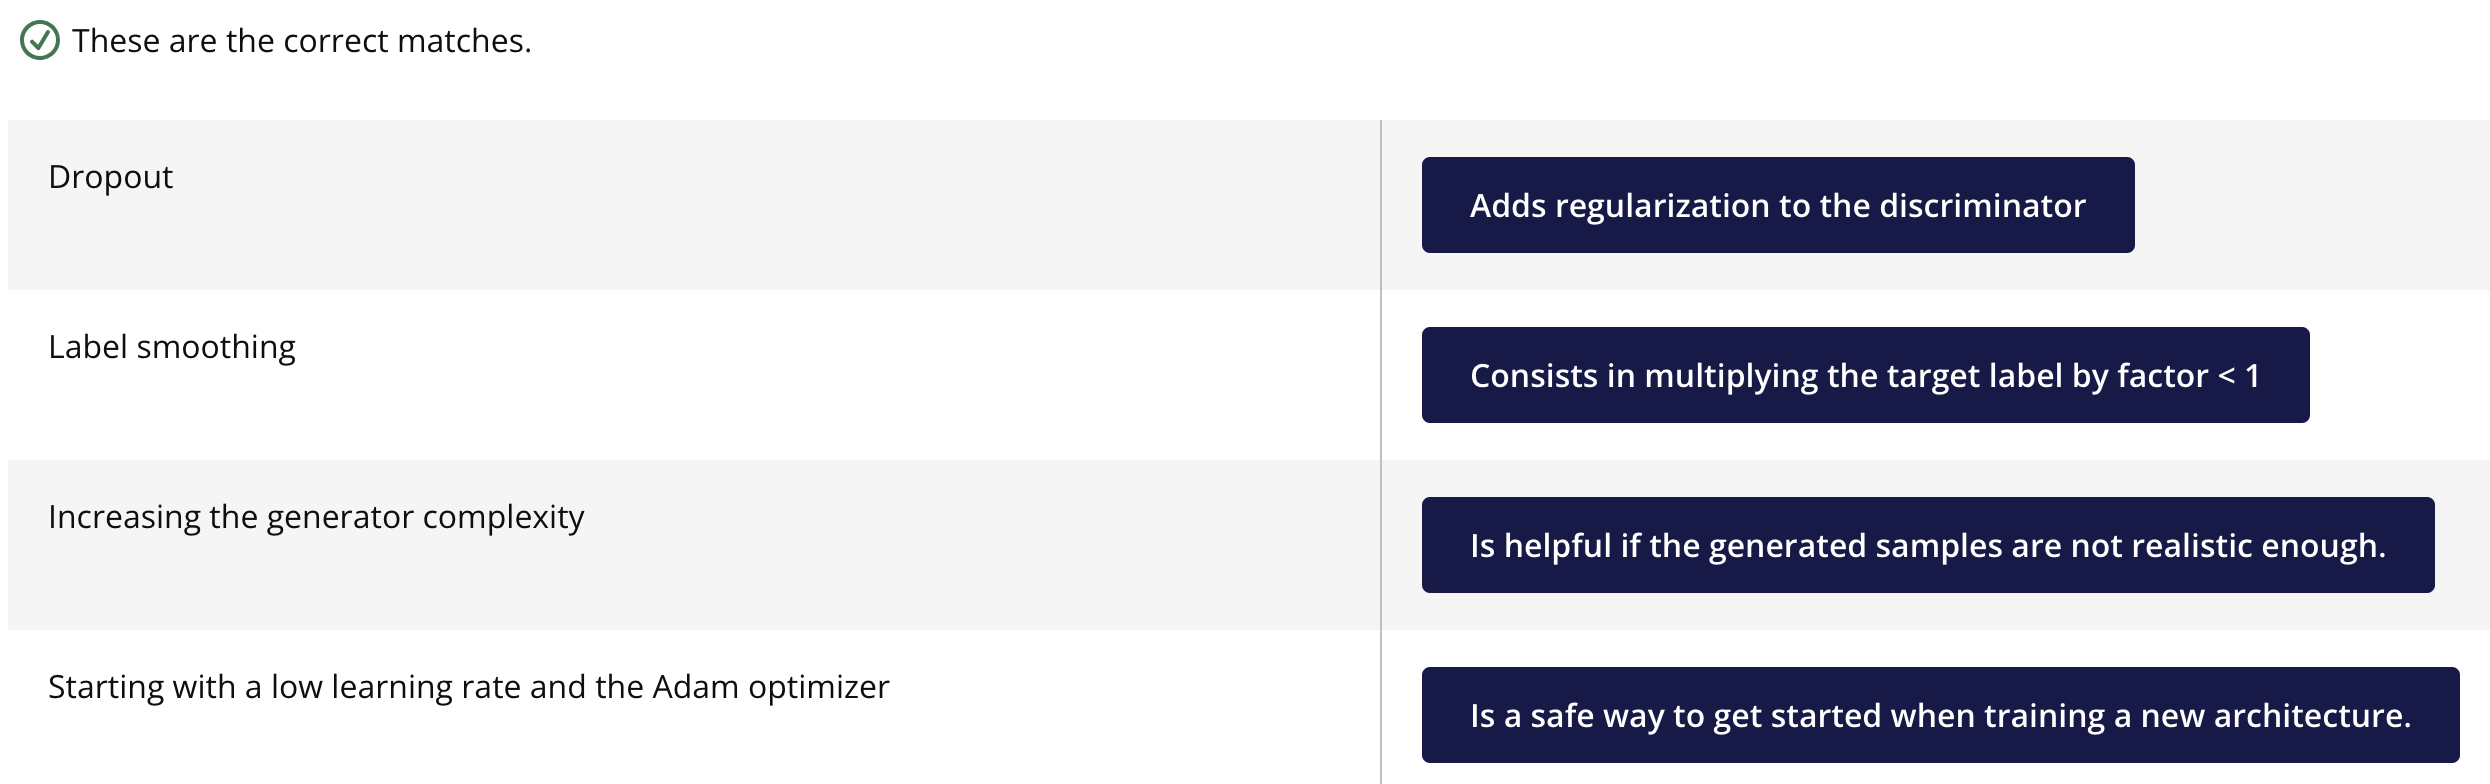
\includegraphics[width=1\linewidth]{img//genAdvNet//deepGAN/quiz2of2.png}
\section{Deep Convolutional GANs}

In this notebook, you'll build a GAN using convolutional layers in the
generator and discriminator. This is called a Deep Convolutional GAN, or
DCGAN for short. The DCGAN architecture was first explored in 2016 and
has seen impressive results in generating new images; you can read the
\href{https://arxiv.org/pdf/1511.06434.pdf}{original paper, here}.

You'll be training DCGAN on the
\href{https://www.cs.toronto.edu/~kriz/cifar.html}{CIFAR10} dataset.
These are color images of different classes, such as airplanes, dogs or
trucks. This dataset is much more complex and diverse than the MNIST
dataset and justifies the use of the DCGAN architecture.

So, our goal is to create a DCGAN that can generate new,
realistic-looking images. We'll go through the following steps to do
this: 
\begin{itemize}
    \item \textbf{Load in and pre-process the CIFAR10 dataset}
    \item Define discriminator and generator networks
    \item \textbf{Train these adversarial networks}
    \item ƒ\textbf{Visualize the loss over time and some sample, generated images}
\end{itemize}

In this notebook, we will focus on defining the networks.

\paragraph{Deeper Convolutional Networks}

Since this dataset is more complex than our MNIST data, we'll need a
deeper network to accurately identify patterns in these images and be
able to generate new ones. Specifically, we'll use a series of
convolutional or transpose convolutional layers in the discriminator and
generator. It's also necessary to use batch normalization to get these
convolutional networks to train.

Besides these changes in network structure, training the discriminator
and generator networks should be the same as before. That is, the
discriminator will alternate training on real and fake (generated)
images, and the generator will aim to trick the discriminator into
thinking that its generated images are real!

\begin{lstlisting}[language=Python]
# # run this cell once to install the dependency. 
# You will have to restart the kernel once the package is installed.
# !pip install ipywidgets
\end{lstlisting}

\begin{lstlisting}[language=Python]
# import libraries
import matplotlib.pyplot as plt
import numpy as np
import pickle as pkl

%matplotlib inline
\end{lstlisting}

\subsection{Getting the data}

Here you can download the CIFAR10 dataset. It's a dataset built-in to
the PyTorch datasets library. We can load in training data, transform it
into Tensor datatypes, then create dataloaders to batch our data into a
desired size.

\begin{lstlisting}[language=Python]
import torch
from torchvision import datasets
from torchvision import transforms

# Tensor transform
transform = transforms.ToTensor()

# CIFAR training datasets
cifar_train = datasets.CIFAR10(root='data/', train=True, download=True, transform=transform)

batch_size = 128
num_workers = 4

# build DataLoaders for CIFAR10 dataset
train_loader = torch.utils.data.DataLoader(dataset=cifar_train,
                                          batch_size=batch_size,
                                          shuffle=True,
                                          num_workers=num_workers)
\end{lstlisting}

\subsubsection{Visualize the Data}

Here I'm showing a small sample of the images. Each of these is 32x32
with 3 color channels (RGB). These are the real, training images that
we'll pass to the discriminator. Notice that each image has \emph{one}
associated, numerical label.

\begin{lstlisting}[language=Python]
# obtain one batch of training images
dataiter = iter(train_loader)
images, labels = dataiter.next()

# plot the images in the batch, along with the corresponding labels
fig = plt.figure(figsize=(25, 4))
plot_size=20
for idx in np.arange(plot_size):
    ax = fig.add_subplot(2, plot_size/2, idx+1, xticks=[], yticks=[])
    ax.imshow(np.transpose(images[idx], (1, 2, 0)))
    # print out the correct label for each image
    # .item() gets the value contained in a Tensor
    ax.set_title(str(labels[idx].item()))
\end{lstlisting}

\subsubsection{Pre-processing: scaling from -1 to 1}

We need to do a bit of pre-processing; we know that the output of our
\lstinline{tanh} activated generator will contain pixel
values in a range from -1 to 1, and so, we need to rescale our training
images to a range of -1 to 1. (Right now, they are in a range from 0-1.)

\begin{lstlisting}[language=Python]
# current range
img = images[0]

print('Min: ', img.min())
print('Max: ', img.max())
\end{lstlisting}

\begin{lstlisting}[language=Python]
# helper scale function
def scale(x, feature_range=(-1, 1)):
    ''' Scale takes in an image x and returns that image, scaled
       with a feature_range of pixel values from -1 to 1. 
       This function assumes that the input x is already scaled from 0-1.'''
    # assume x is scaled to (0, 1)
    # scale to feature_range and return scaled x
    min_val, max_val = feature_range
    x = x * (max_val - min_val) + min_val
    return x
\end{lstlisting}

\begin{lstlisting}[language=Python]
# scaled range
scaled_img = scale(img)

print('Scaled min: ', scaled_img.min())
print('Scaled max: ', scaled_img.max())
\end{lstlisting}

\section{Define the Model}

A GAN is comprised of two adversarial networks, a discriminator and a
generator. Let's use the models we created in the previous exercise.

\subsection{Discriminator}

Here you'll build the discriminator. This is a convolutional classifier
like you've built before, only without any maxpooling layers. 
\begin{itemize}
    \item The inputs to the discriminator are 32x32x3 tensor images
    \item You'll want a few convolutional, hidden layers
    \item Then a fully connected layer for the output; as before, we want a sigmoid output, but we'll add that in the loss function, \href{https://pytorch.org/docs/stable/nn.html\#bcewithlogitsloss}{BCEWithLogitsLoss}, later
\end{itemize}

\begin{lstlisting}[language=Python]
import torch.nn as nn
\end{lstlisting}

\begin{lstlisting}[language=Python]
class ConvBlock(nn.Module):
    """
    A convolutional block is made of 3 layers: Conv -> BatchNorm -> Activation.
    args:
    - in_channels: number of channels in the input to the conv layer
    - out_channels: number of filters in the conv layer
    - kernel_size: filter dimension of the conv layer
    - batch_norm: whether to use batch norm or not
    """
    def __init__(self, in_channels: int, out_channels: int, kernel_size: int, batch_norm: bool = True):
        super(ConvBlock, self).__init__()
        
        self.conv = nn.Conv2d(in_channels, out_channels, kernel_size, stride=2, padding=1, bias=False)
        self.batch_norm = batch_norm
        if self.batch_norm:
            self.bn = nn.BatchNorm2d(out_channels)
        self.activation = nn.LeakyReLU(0.2)
        
    def forward(self, x: torch.Tensor) -> torch.Tensor:
        x = self.conv(x)
        if self.batch_norm:
            x = self.bn(x)
        x = self.activation(x)
        return x
\end{lstlisting}

\begin{lstlisting}[language=Python]
class Discriminator(nn.Module):
    """
    The discriminator model adapted from the DCGAN paper. It should only contains a few layers.
    args:
    - conv_dim: control the number of filters
    """
    def __init__(self, conv_dim: int):
        super(Discriminator, self).__init__()

        # complete init function
        self.conv_dim = conv_dim

        # 32x32 input
        self.conv1 = ConvBlock(3, conv_dim, 4, batch_norm=False) # first layer, no batch_norm
        # 16x16 out
        self.conv2 = ConvBlock(conv_dim, conv_dim*2, 4)
        # 8x8 out
        self.conv3 = ConvBlock(conv_dim*2, conv_dim*4, 4)
        # 4x4 out
        
        self.flatten = nn.Flatten()
        # final, fully-connected layer
        self.fc = nn.Linear(conv_dim*4*4*4, 1)

    def forward(self, x):
        # all hidden layers + leaky relu activation
        x = self.conv1(x)
        x = self.conv2(x)
        x = self.conv3(x)
        # flatten
        x = self.flatten(x)
        # final output layer
        x = self.fc(x)        
        return x
\end{lstlisting}

\subsection{Generator}

Next, you'll build the generator network. The input will be our noise
vector \lstinline{z}, as before. And, the output will be a
\(tanh\) output, but this time with size 32x32 which is the size of our
CIFAR10 images.

\begin{lstlisting}[language=Python]
class DeconvBlock(nn.Module):
    """
    A "de-convolutional" block is made of 3 layers: ConvTranspose -> BatchNorm -> Activation.
    args:
    - in_channels: number of channels in the input to the conv layer
    - out_channels: number of filters in the conv layer
    - kernel_size: filter dimension of the conv layer
    - stride: stride of the conv layer
    - padding: padding of the conv layer
    - batch_norm: whether to use batch norm or not
    """
    def __init__(self, 
                 in_channels: int, 
                 out_channels: int, 
                 kernel_size: int, 
                 stride: int,
                 padding: int,
                 batch_norm: bool = True):
        super(DeconvBlock, self).__init__()
        self.deconv = nn.ConvTranspose2d(in_channels, out_channels, kernel_size, stride, padding, bias=False)
        self.batch_norm = batch_norm
        if self.batch_norm:
            self.bn = nn.BatchNorm2d(out_channels)
        self.activation = nn.ReLU()
        
    def forward(self, x: torch.Tensor) -> torch.Tensor:
        x = self.deconv(x)
        if self.batch_norm:
            x = self.bn(x)
        x = self.activation(x)
        return x
\end{lstlisting}

\begin{lstlisting}[language=Python]
class Generator(nn.Module):
    """
    The generator model adapted from DCGAN
    args:
    - latent_dim: dimension of the latent vector
    - conv_dim: control the number of filters in the convtranspose layers
    """
    def __init__(self, latent_dim: int, conv_dim: int = 32):
        super(Generator, self).__init__()
        # transpose conv layers
        self.deconv1 = DeconvBlock(latent_dim, conv_dim*4, 4, 1, 0)
        self.deconv2 = DeconvBlock(conv_dim*4, conv_dim*2, 4, 2, 1)
        self.deconv3 = DeconvBlock(conv_dim*2, conv_dim, 4, 2, 1)
        self.deconv4 = nn.ConvTranspose2d(conv_dim, 3, 4, stride=2, padding=1)
        self.last_activation = nn.Tanh()
        
    def forward(self, x):
        x = self.deconv1(x)
        x = self.deconv2(x)
        x = self.deconv3(x)
        x = self.deconv4(x)
        x = self.last_activation(x)
        return x
    
\end{lstlisting}

\subsection{Build complete network}

Define your models' hyperparameters and instantiate the discriminator
and generator from the classes defined above. Make sure you've passed in
the correct input arguments.

\begin{lstlisting}[language=Python]
# define hyperparams
conv_dim = 32
z_size = 100

# define discriminator and generator
D = Discriminator(conv_dim)
G = Generator(latent_dim=z_size, conv_dim=conv_dim)
\end{lstlisting}

\subsubsection{Training on GPU}

Check if you can train on GPU. If you can, set this as a variable and
move your models to GPU. \textgreater{} Later, we'll also move any
inputs our models and loss functions see (real\_images, z, and ground
truth labels) to GPU as well.

\begin{lstlisting}[language=Python]
train_on_gpu = torch.cuda.is_available()

if train_on_gpu:
    # move models to GPU
    G.cuda()
    D.cuda()
    print('GPU available for training. Models moved to GPU')
else:
    print('Training on CPU.')
    
\end{lstlisting}

\subsection{Discriminator and Generator Losses}

Now we need to calculate the losses. And this will be exactly the same
as before.

\subsubsection{Discriminator Losses}

\begin{quote}
\begin{itemize}
\item For the discriminator, the total loss is the sum of the losses for real and fake images,  \lstinline{d_loss = d_real_loss + d_fake_loss}.
\item Remember that we want the discriminator to output 1 for real images and 0 for fake images, so we need to set up the losses to reflect that.
\end{itemize}
\end{quote}

The losses will by binary cross entropy loss with logits, which we can
get with
\href{https://pytorch.org/docs/stable/nn.html\#bcewithlogitsloss}{BCEWithLogitsLoss}.
This combines a \lstinline{sigmoid} activation function
\textbf{and} binary cross entropy loss in one function.

For the real images, we want
\lstinline{D(real_images) = 1}. That is, we want the
discriminator to classify the real images with a label = 1, indicating
that these are real. The discriminator loss for the fake data is
similar. We want \lstinline{D(fake_images) = 0}, where
the fake images are the \emph{generator output},
\lstinline{fake_images = G(z)}.

\subsubsection{Generator Loss}

The generator loss will look similar only with flipped labels. The
generator's goal is to get
\lstinline{D(fake_images) = 1}. In this case, the labels
are \textbf{flipped} to represent that the generator is trying to fool
the discriminator into thinking that the images it generates (fakes) are
real!

\begin{lstlisting}[language=Python]
def real_loss(D_out, smooth=False):
    batch_size = D_out.size(0)
    # label smoothing
    if smooth:
        # smooth, real labels = 0.9
        labels = torch.ones(batch_size)*0.9
    else:
        labels = torch.ones(batch_size) # real labels = 1
    # move labels to GPU if available     
    if train_on_gpu:
        labels = labels.cuda()
    # binary cross entropy with logits loss
    criterion = nn.BCEWithLogitsLoss()
    # calculate loss
    loss = criterion(D_out.squeeze(), labels)
    return loss

def fake_loss(D_out):
    batch_size = D_out.size(0)
    labels = torch.zeros(batch_size) # fake labels = 0
    if train_on_gpu:
        labels = labels.cuda()
    criterion = nn.BCEWithLogitsLoss()
    # calculate loss
    loss = criterion(D_out.squeeze(), labels)
    return loss
\end{lstlisting}

\subsection{Optimizers}

Not much new here, but notice how I am using a small learning rate and
custom parameters for the Adam optimizers, This is based on some
research into DCGAN model convergence.

\subsubsection{Hyperparameters}

GANs are very sensitive to hyperparameters. A lot of experimentation
goes into finding the best hyperparameters such that the generator and
discriminator don't overpower each other. Try out your own
hyperparameters or read \href{https://arxiv.org/pdf/1511.06434.pdf}{the
DCGAN paper} to see what worked for them.

\begin{lstlisting}[language=Python]
import torch.optim as optim

# params
lr = 0.0002
beta1=0.5
beta2=0.999 # default value

# Create optimizers for the discriminator and generator
d_optimizer = optim.Adam(D.parameters(), lr, [beta1, beta2])
g_optimizer = optim.Adam(G.parameters(), lr, [beta1, beta2])
\end{lstlisting}

\subsection{Training}

Training will involve alternating between training the discriminator and
the generator. We'll use our functions
\lstinline{real_loss} and
\lstinline{fake_loss} to help us calculate the
discriminator losses in all of the following cases.

\subsubsection{Discriminator training}

\begin{enumerate}
\item Compute the discriminator loss on real, training images\\
\item Generate fake images
\item Compute the discriminator loss on fake, generated images\\
\item Add up real and fake loss
\item Perform backpropagation + an optimization step to update the discriminator's weights
\end{enumerate}

\subsubsection{Generator training}

\begin{enumerate}
\item Generate fake images
\item Compute the discriminator loss on fake images, using \textbf{flipped} labels!
\item Perform backpropagation + an optimization step to update the generator's weights
\end{enumerate}

\paragraph{Saving Samples}

As we train, we'll also print out some loss statistics and save some
generated ``fake'' samples.

\textbf{Evaluation mode}

Notice that, when we call our generator to create the samples to
display, we set our model to evaluation mode:
\lstinline{G.eval()}. That's so the batch normalization
layers will use the population statistics rather than the batch
statistics (as they do during training), \emph{and} so dropout layers
will operate in eval() mode; not turning off any nodes for generating
samples.

\begin{lstlisting}[language=Python]
import pickle as pkl
from datetime import datetime
\end{lstlisting}

\begin{lstlisting}[language=Python]
# helper function for viewing a list of passed in sample images
def view_samples(epoch, samples):
    fig, axes = plt.subplots(figsize=(14,4), nrows=2, ncols=8, sharey=True, sharex=True)
    for ax, img in zip(axes.flatten(), samples[epoch]):
        img = img.detach().cpu().numpy()
        img = np.transpose(img, (1, 2, 0))
        img = ((img +1)*255 / (2)).astype(np.uint8) # rescale to pixel range (0-255)
        ax.xaxis.set_visible(False)
        ax.yaxis.set_visible(False)
        im = ax.imshow(img.reshape((32,32,3)))
    plt.show()
\end{lstlisting}

\begin{lstlisting}[language=Python]
# training hyperparams
num_epochs = 10

# keep track of loss and generated, "fake" samples
samples = []
losses = []

print_every = 100

# Get some fixed data for sampling. These are images that are held
# constant throughout training, and allow us to inspect the model's performance
sample_size=16
fixed_z = np.random.uniform(-1, 1, size=(sample_size, z_size, 1, 1))
fixed_z = torch.from_numpy(fixed_z).float()

# train the network
for epoch in range(num_epochs):
    
    for batch_i, (real_images, _) in enumerate(train_loader):
                
        batch_size = real_images.size(0)
        
        # important rescaling step
        real_images = scale(real_images)
        
        # ============================================
        #            TRAIN THE DISCRIMINATOR
        # ============================================
        
        d_optimizer.zero_grad()
        
        # 1. Train with real images

        # Compute the discriminator losses on real images 
        if train_on_gpu:
            real_images = real_images.cuda()
        
        D_real = D(real_images)
        d_real_loss = real_loss(D_real)
        
        # 2. Train with fake images
        
        # Generate fake images
        z = np.random.uniform(-1, 1, size=(batch_size, z_size, 1, 1))
        z = torch.from_numpy(z).float()
        # move x to GPU, if available
        if train_on_gpu:
            z = z.cuda()
        fake_images = G(z)
        
        # Compute the discriminator losses on fake images            
        D_fake = D(fake_images.detach())
        d_fake_loss = fake_loss(D_fake)
        
        # add up loss and perform backprop
        d_loss = d_real_loss + d_fake_loss
        d_loss.backward()
        d_optimizer.step()
        
        
        # =========================================
        #            TRAIN THE GENERATOR
        # =========================================
        g_optimizer.zero_grad()
        
        # 1. Train with fake images and flipped labels
        
        # Generate fake images
        z = np.random.uniform(-1, 1, size=(batch_size, z_size, 1, 1))
        z = torch.from_numpy(z).float()
        if train_on_gpu:
            z = z.cuda()
        fake_images = G(z)
        
        # Compute the discriminator losses on fake images 
        # using flipped labels!
        D_fake = D(fake_images)
        g_loss = real_loss(D_fake) # use real loss to flip labels
        
        # perform backprop
        g_loss.backward()
        g_optimizer.step()

        # Print some loss stats
        if batch_i % print_every == 0:
            # append discriminator loss and generator loss
            losses.append((d_loss.item(), g_loss.item()))
            # print discriminator and generator loss
            time = str(datetime.now()).split('.')[0]
            print(f'{time} | Epoch [{epoch+1}/{num_epochs}] | Batch {batch_i}/{len(train_loader)} | d_loss: {d_loss.item():.4f} | g_loss: {g_loss.item():.4f}')
    
    ## AFTER EACH EPOCH##    
    # generate and save sample, fake images
    G.eval() # for generating samples
    if train_on_gpu:
        fixed_z = fixed_z.cuda()
    samples_z = G(fixed_z)
    samples.append(samples_z)
    view_samples(-1, samples)
    G.train() # back to training mode


# Save training generator samples
with open('train_samples.pkl', 'wb') as f:
    pkl.dump(samples, f)
\end{lstlisting}

\subsection{Training loss}

Here we'll plot the training losses for the generator and discriminator,
recorded after each epoch.

\begin{lstlisting}[language=Python]
fig, ax = plt.subplots()
losses = np.array(losses)
plt.plot(losses.T[0], label='Discriminator', alpha=0.5)
plt.plot(losses.T[1], label='Generator', alpha=0.5)
plt.title("Training Losses")
plt.legend()
\end{lstlisting}


Solution on \href{https://www.youtube.com/watch?v=uS8L9eW6Jnk&t=1s}{Youtube}

\section{GAN Evaluation}
\href{https://www.youtube.com/watch?v=Dfmdp0CX-yk&t=2s}{Youtube} \newline

BEcause GANs do not have a straightforward way of evaluation, new metrics are needed: Inception Score (IS) and Frechet Inception Distance (FID). Both of these scores use the Inception Model which is a ConvNet using the inception module. The Inception Score relies on the KL divergence.
\subsection{The Inception Model}
The \textbf{Inception Model} is a concatenation of the outputs of layers of different filter sizes that allows deeper networks. The Inception Score and the Frechet Inception use the Inception Model for their calculations.

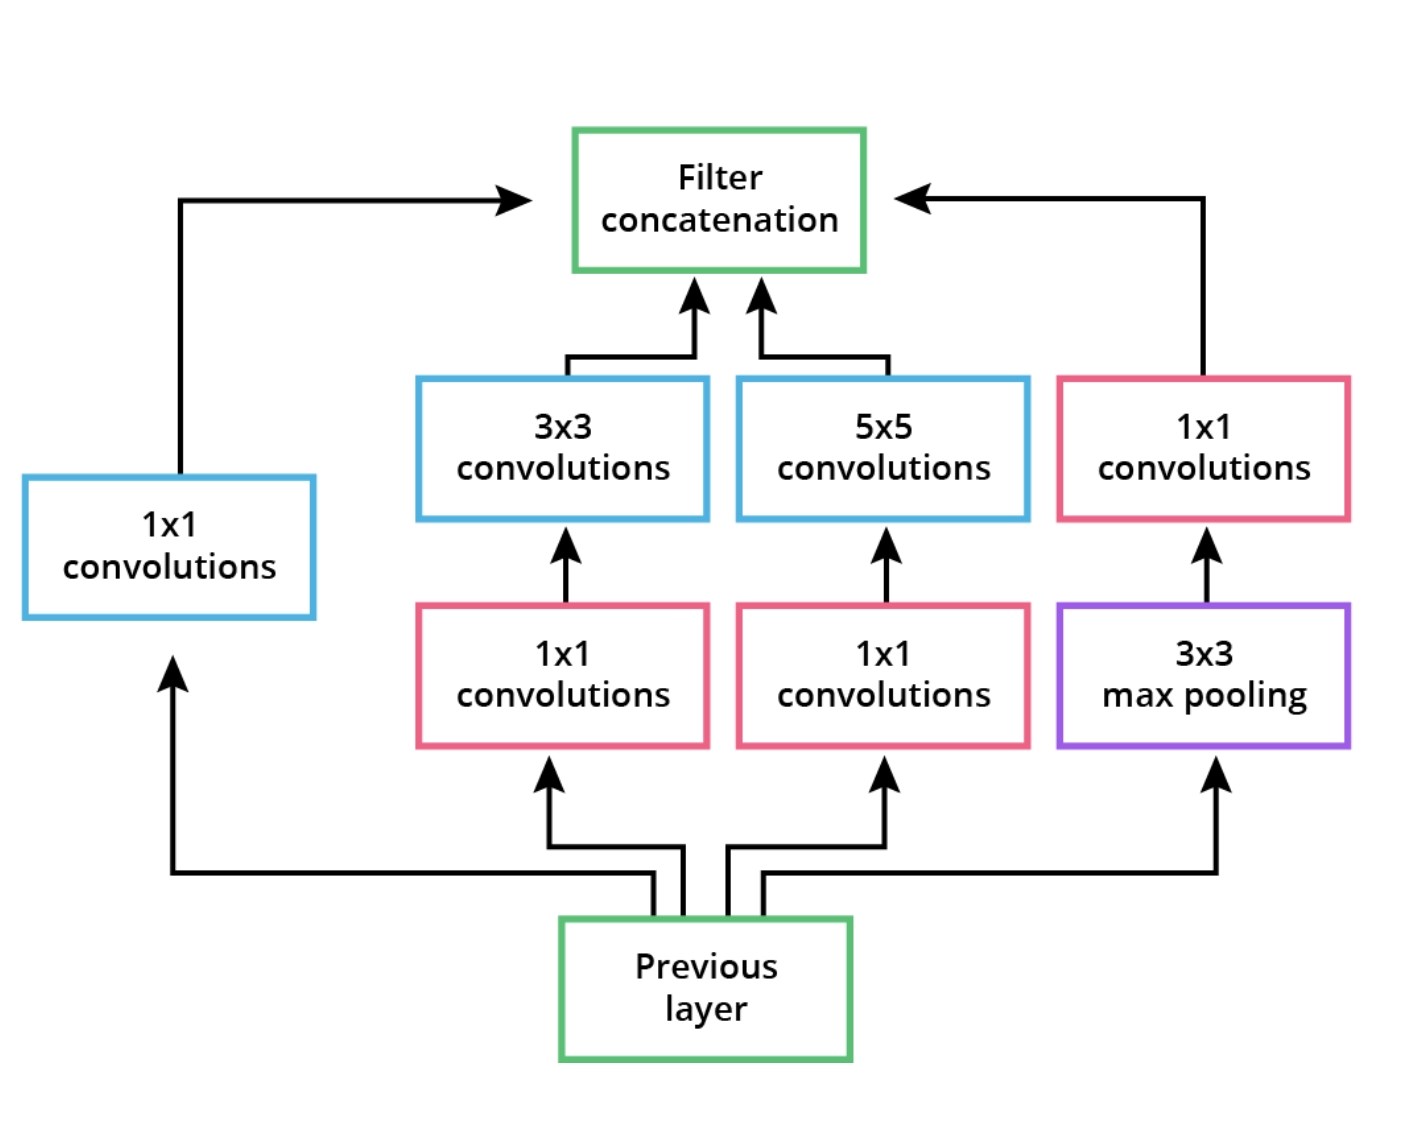
\includegraphics[width=0.5\linewidth]{img//genAdvNet//deepGAN/screen-shot-2022-05-10-at-11.55.59-am.jpeg}
\captionof{figure}{The inception model}


\subsection{Kullback Leibler (KL) Divergence}
The KL divergence is a measure of distance between two probability distributions.

\begin{itemize}
    \item \textbf{Low KL divergence} means that the distributions are similar
    \item \textbf{High KL divergence} means that they are different
\end{itemize}

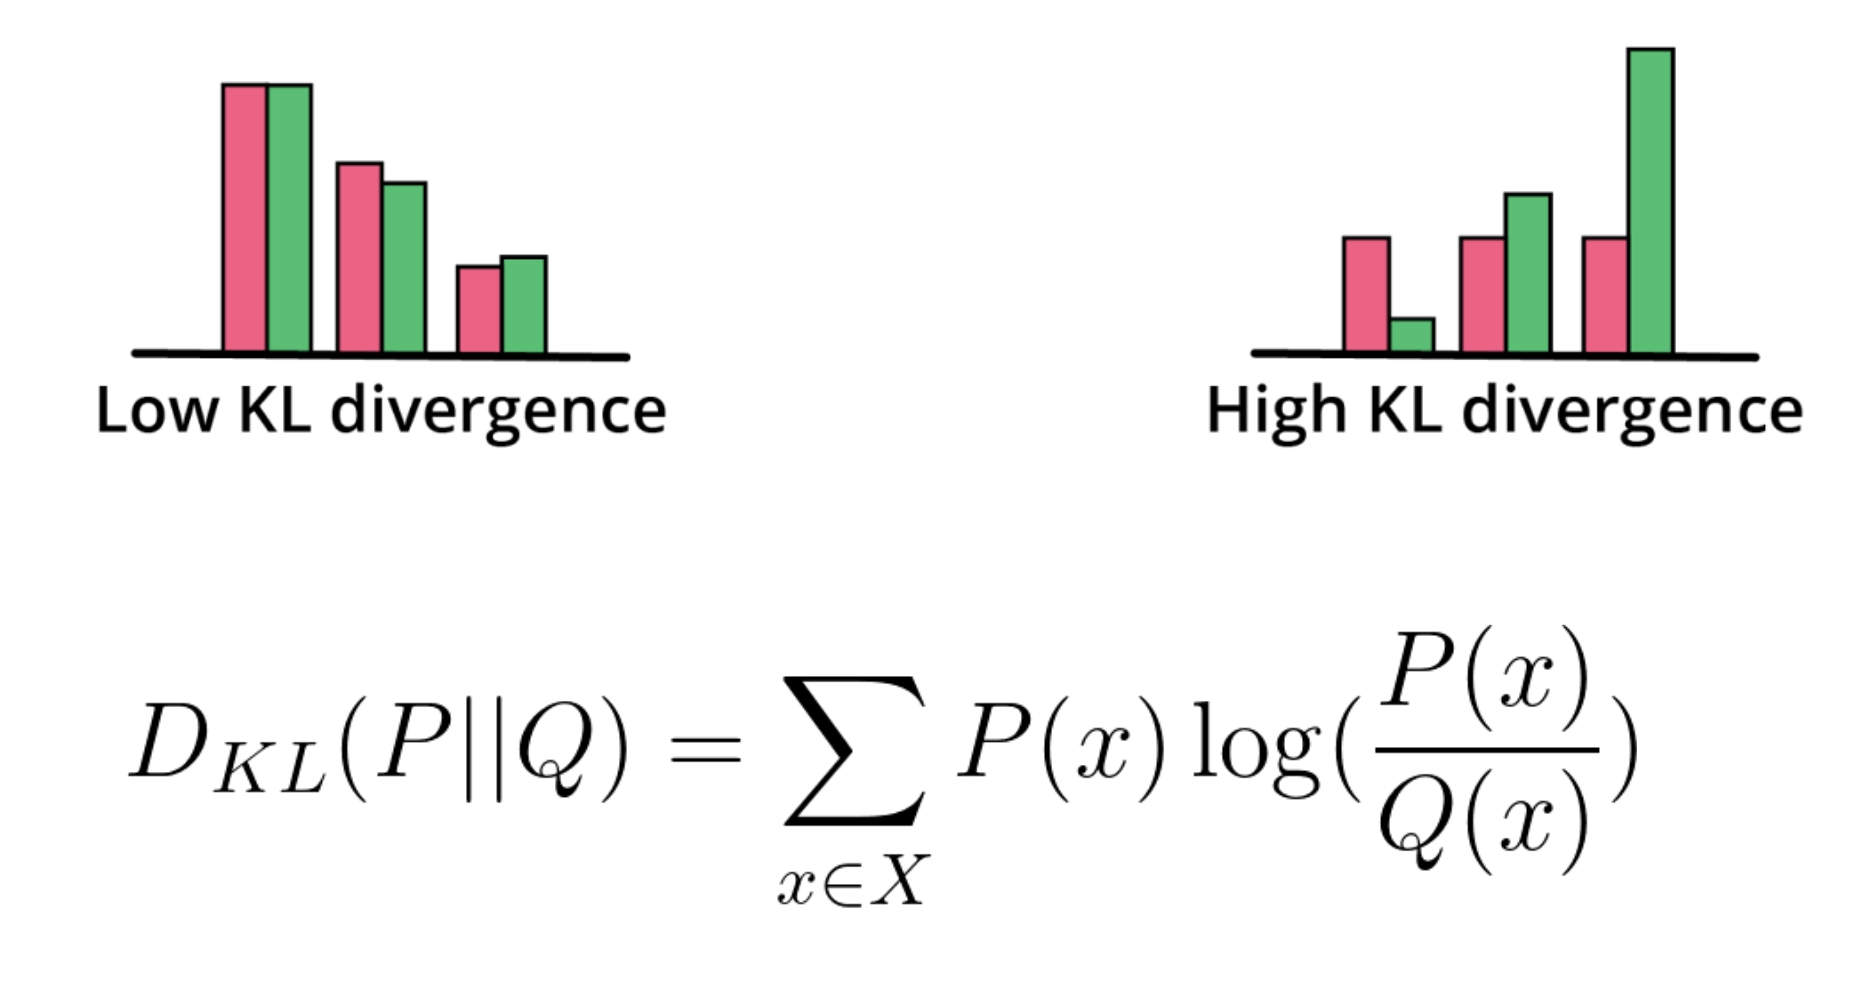
\includegraphics[width=0.5\linewidth]{img//genAdvNet//deepGAN/screen-shot-2022-05-10-at-12.48.18-pm.jpeg}
\captionof{figure}{The Kullback Leibler (KL) divergence}
\section{The Inception Score}
\href{https://www.youtube.com/watch?v=OLnqLdfOpHc}{Youtube} \newline

The \textbf{Inception Score} leverages the KL divergence and the inception model to evaluate generated samples. To calculate the inception score, build two probability distributions.

\begin{enumerate}
    \item \textbf{Conditional Distribution} – feed a generated sample through the inception model pre-trained on the \href{https://www.image-net.org/}{\textbf{ImageNet dataset}}. The inception model will output a probability distribution with the last soft-max layer.
    \item \textbf{Marginal Distribution} – the mean of all the \(p(y|x)\) over all of the \(x\) values.

    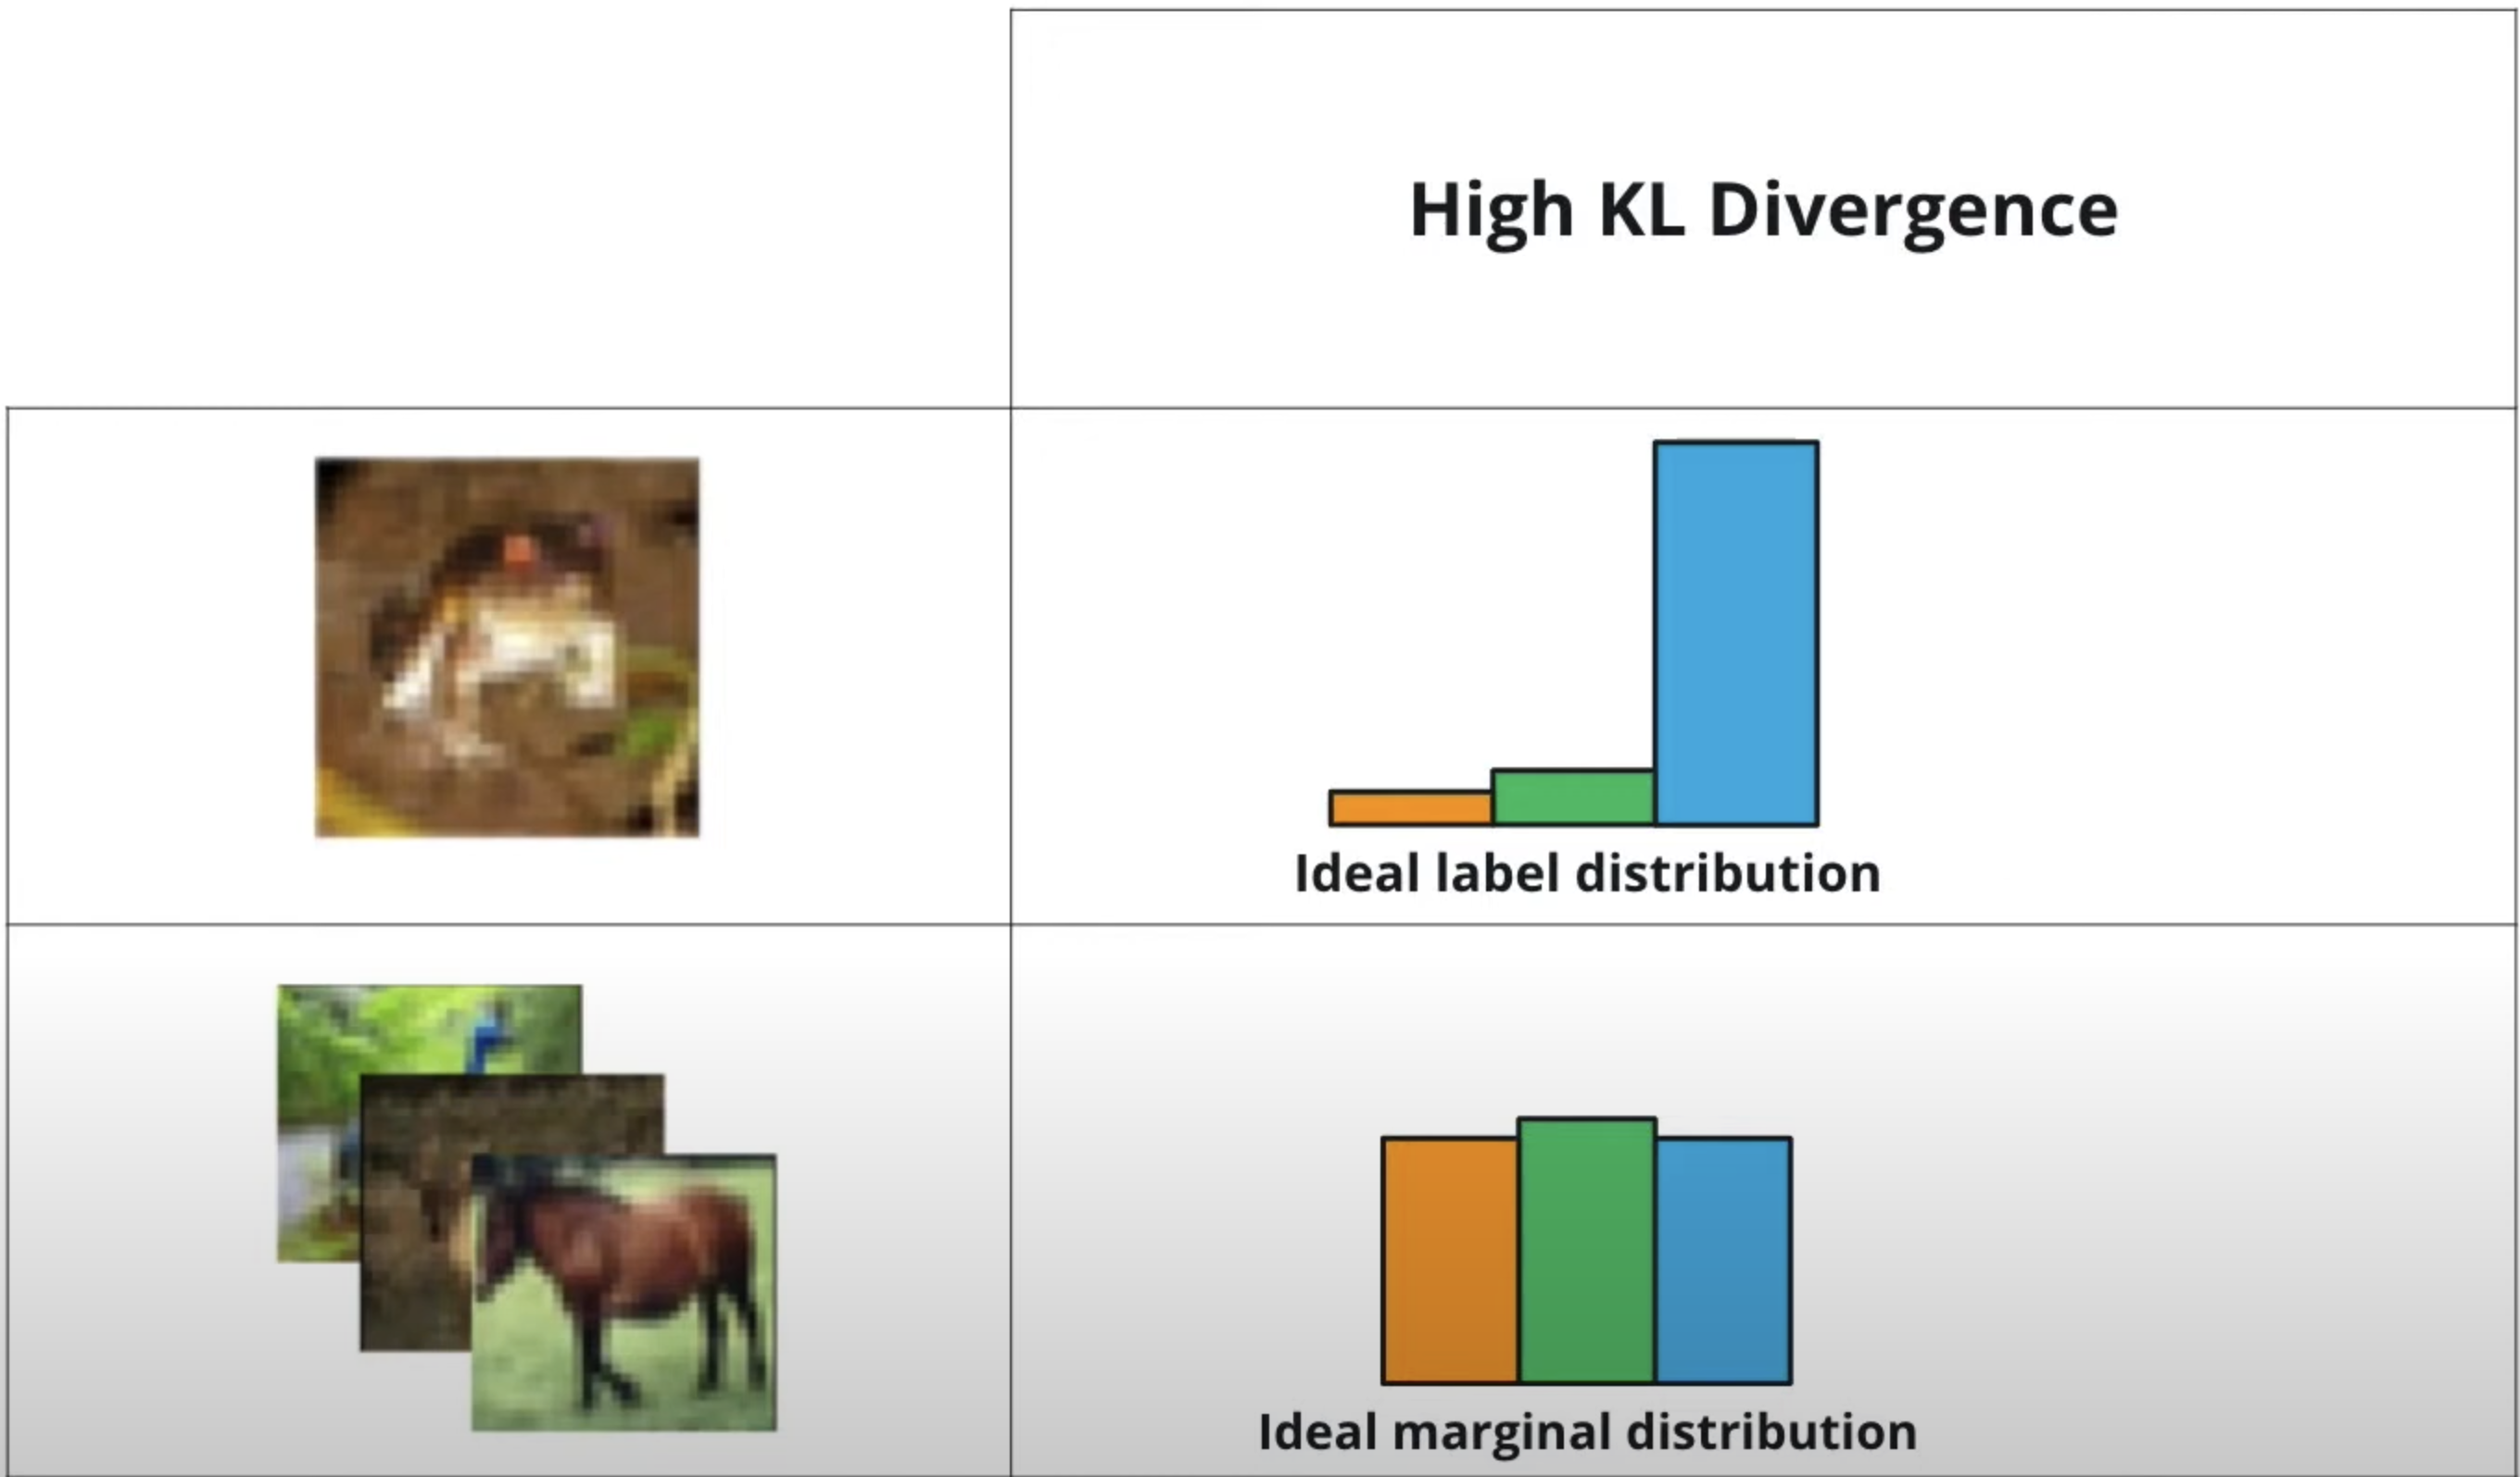
\includegraphics[width=0.5\linewidth]{img//genAdvNet//deepGAN/maeginalDist.png}
    \captionof{figure}{We want our marginal distribution to be somewhat uniform. Hence, averaging over all our samples, no labels are more probable than any other.}
    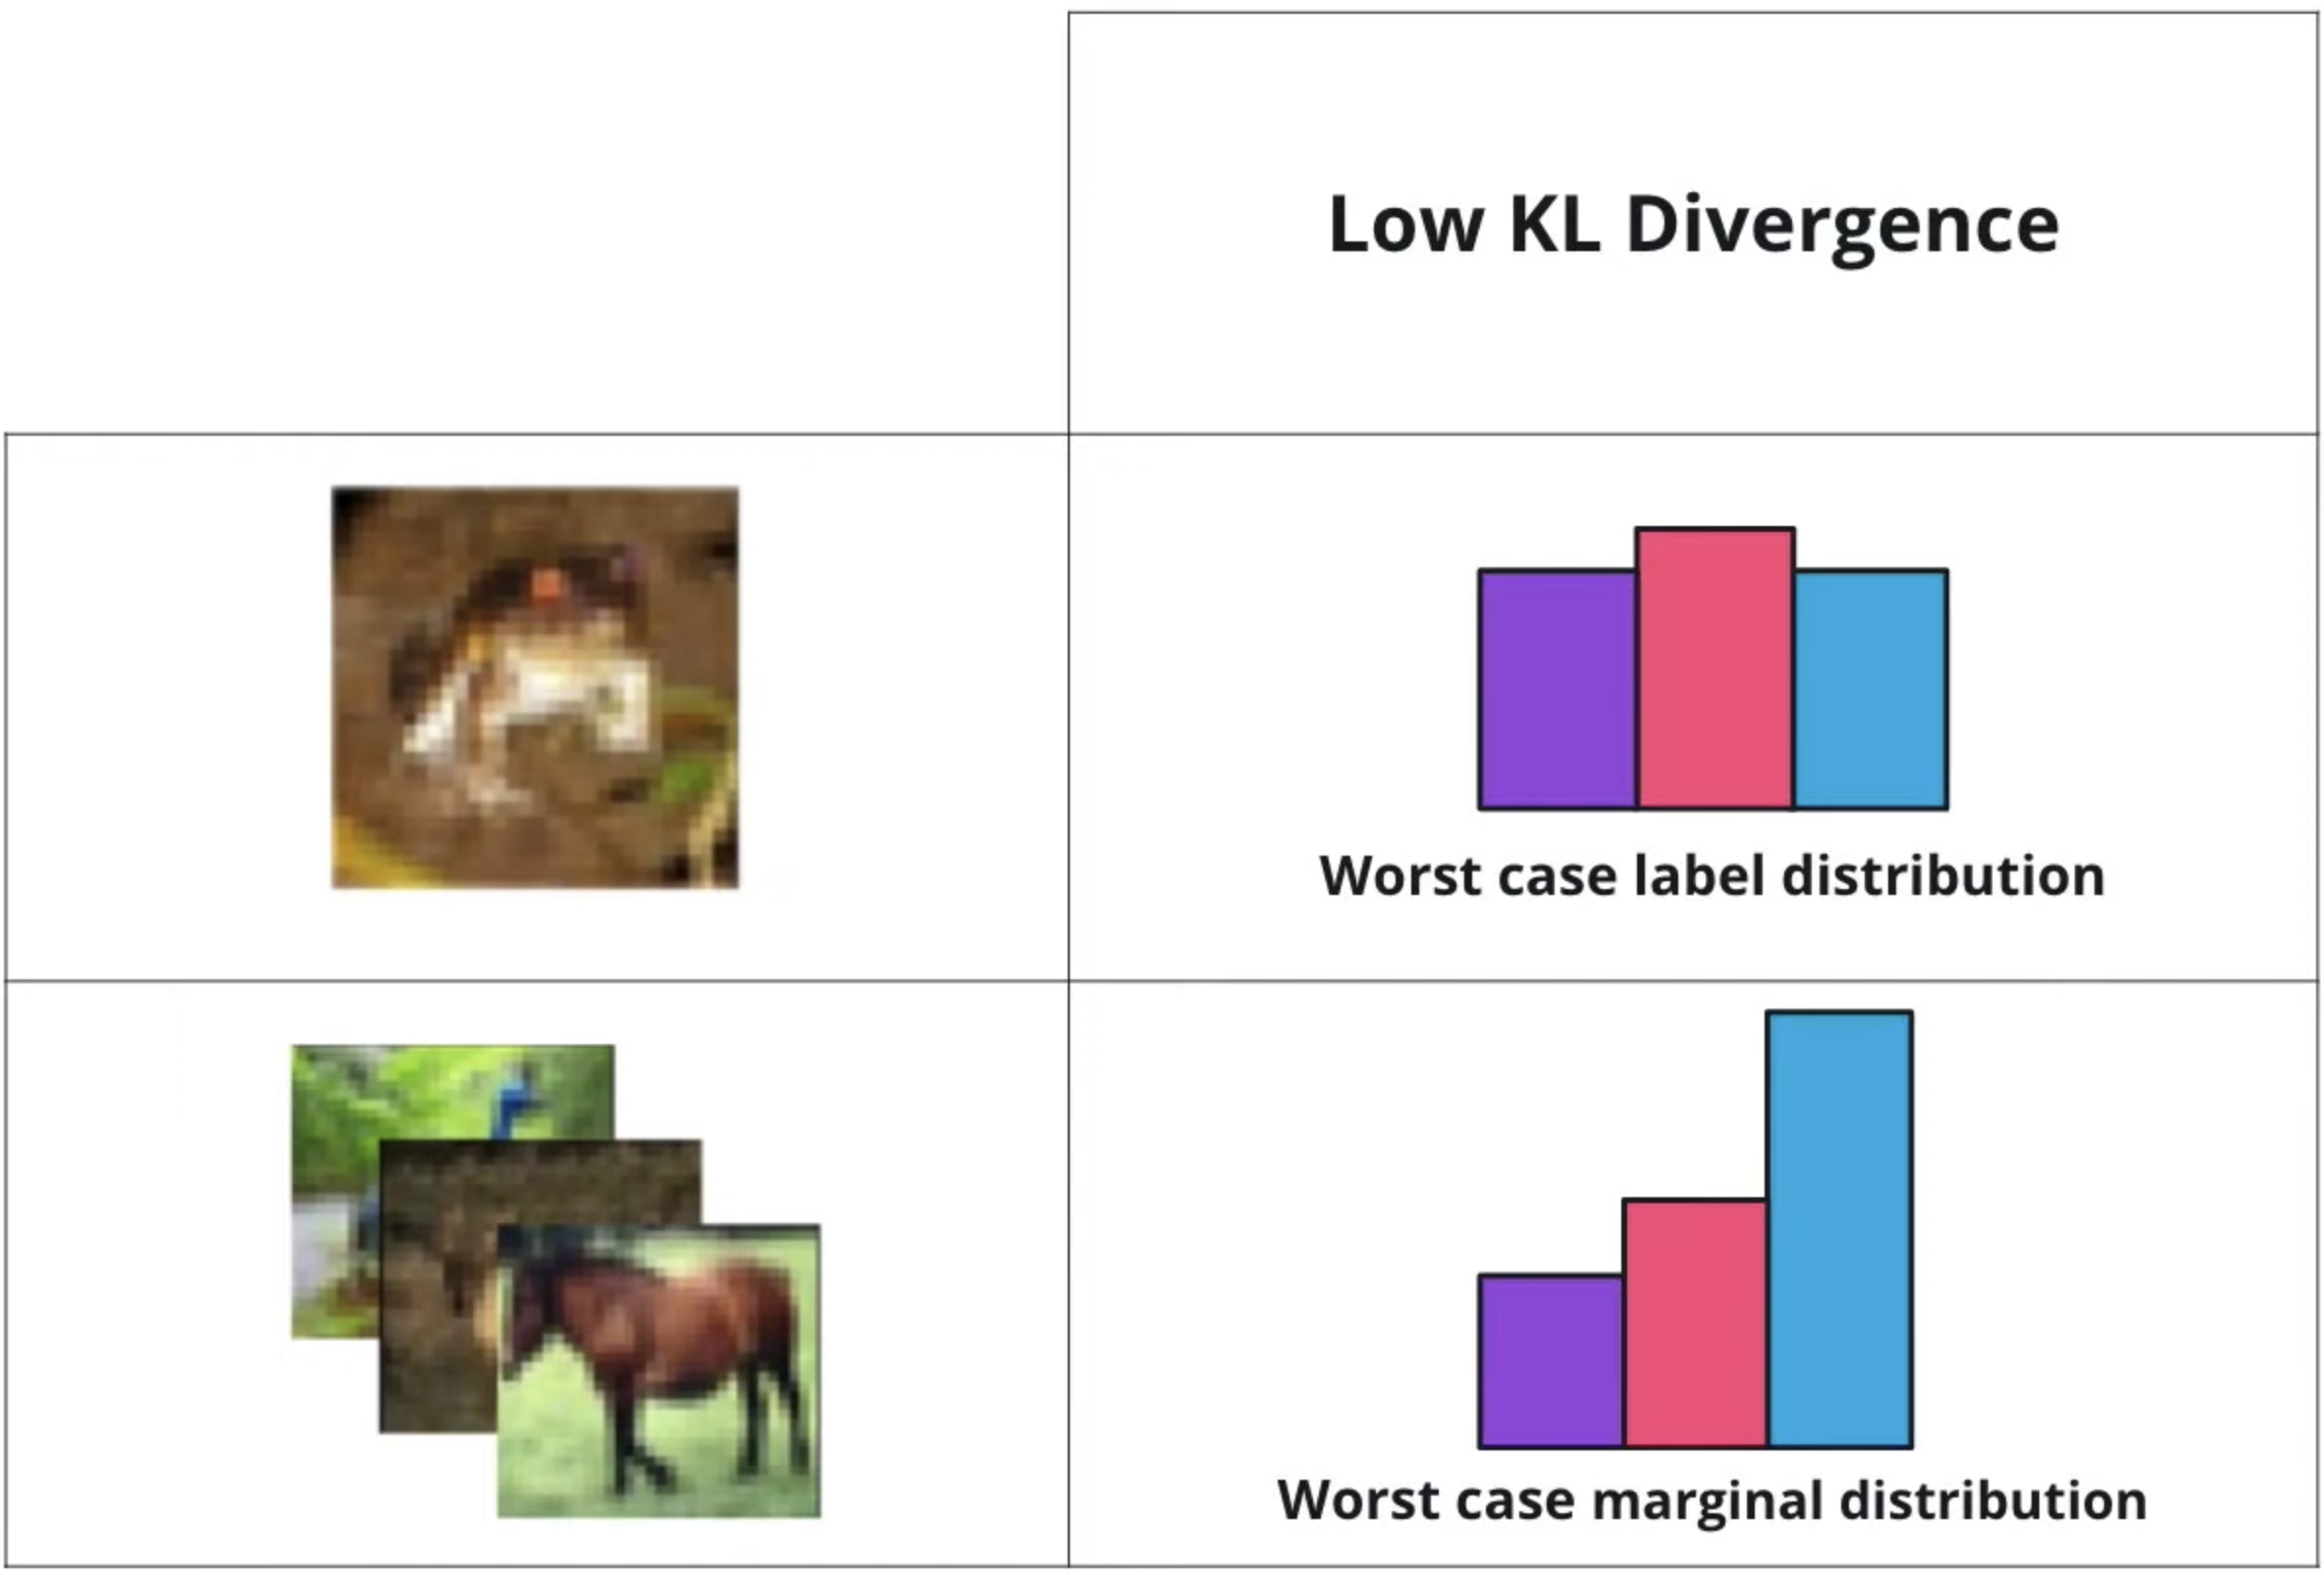
\includegraphics[width=0.5\linewidth]{img//genAdvNet//deepGAN/marginalDistLowKL.png}
    \captionof{figure}{Our model is not very confident on any particular label and does not show diversity.}
    \item Use \textbf{KL Divergence} to measure the distance between the two distributions.
\end{enumerate}

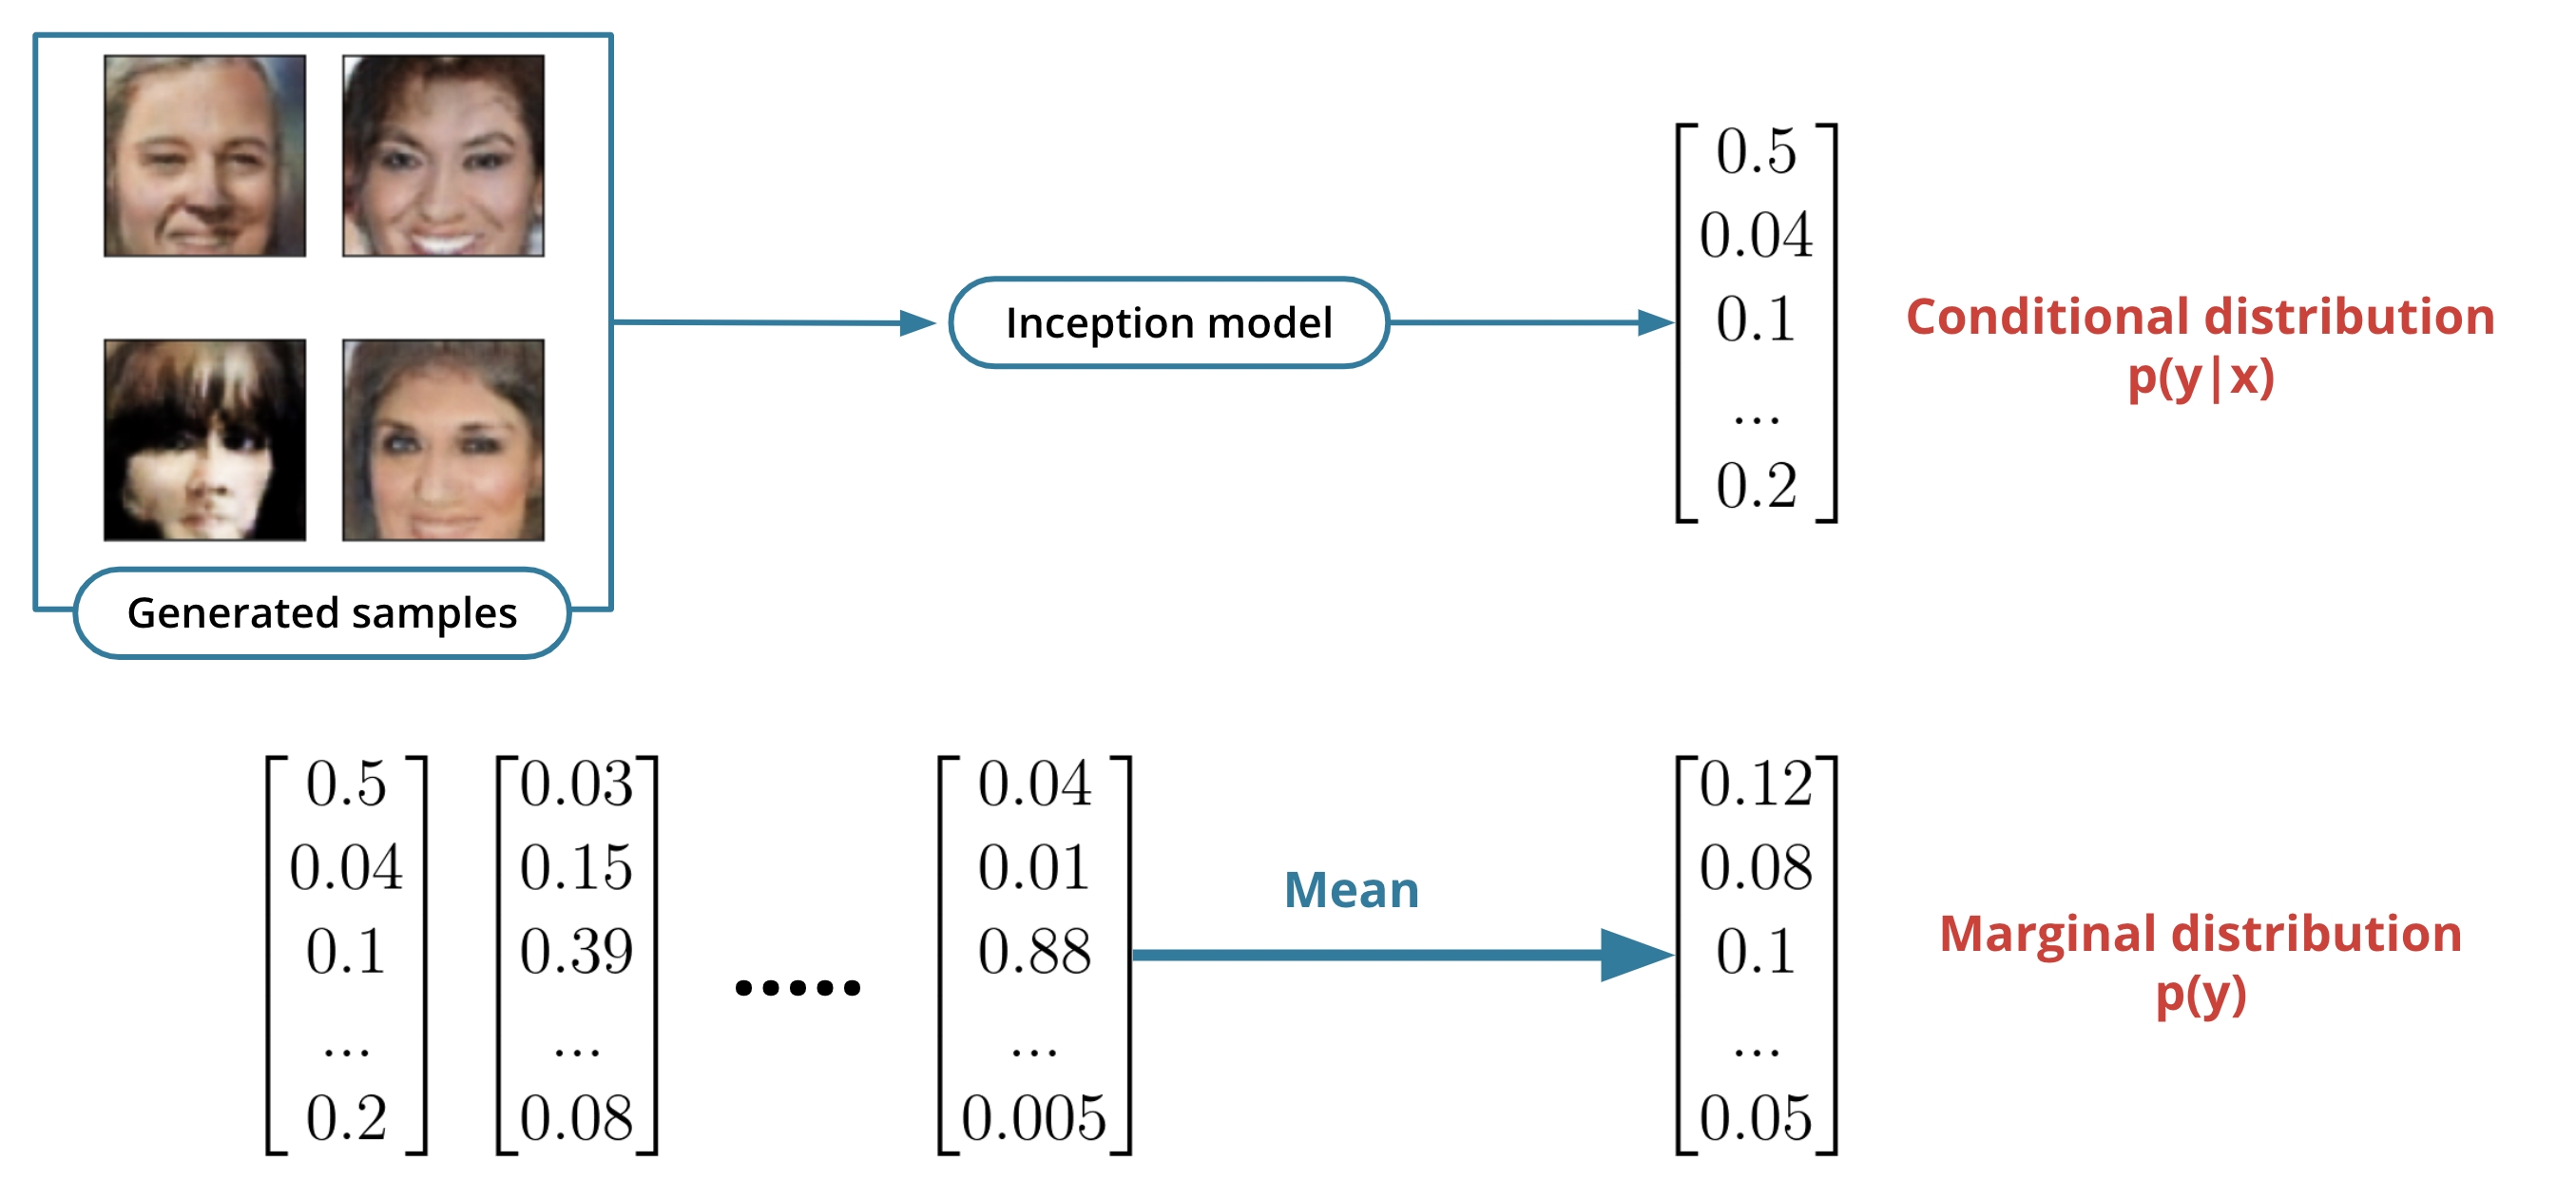
\includegraphics[width=1\linewidth]{img//genAdvNet//deepGAN/screen-shot-2022-05-10-at-2.21.02-pm.jpeg}
\captionof{figure}{Flowchart of how conditional and marginal distributions are generated}

The \textbf{Inception Score} is: \[e^{E[KL(p(y|x), p(y))]}\]
where the exponent is the expected value of KL divergence between the marginal and the conditional label distribution over all the generated samples. \newline

The higher the inception score, the better our generated samples are.
\subsection{Inception Score Limitations}
The inception score is a great tool to calculate a GAN performance but has some limitations:
\begin{itemize}
    \item It relies on a model pre-trained on the ImageNet dataset.
    \item It does not take into account the real dataset, which can be limiting in some situations.
\end{itemize}

\section{Frechet Inception Distance}
Youtube


\begin{itemize}
    \item \(m_f\): mean of the fake distribution
    \item \(C_f\): covariance of the fake distribution
\end{itemize}
\textbf{Frechet Inception Distance} or \textbf{FID} measures the distance between two multinomial Gaussian distributions, where the mean and covariance are calculated from the real and the generated samples.

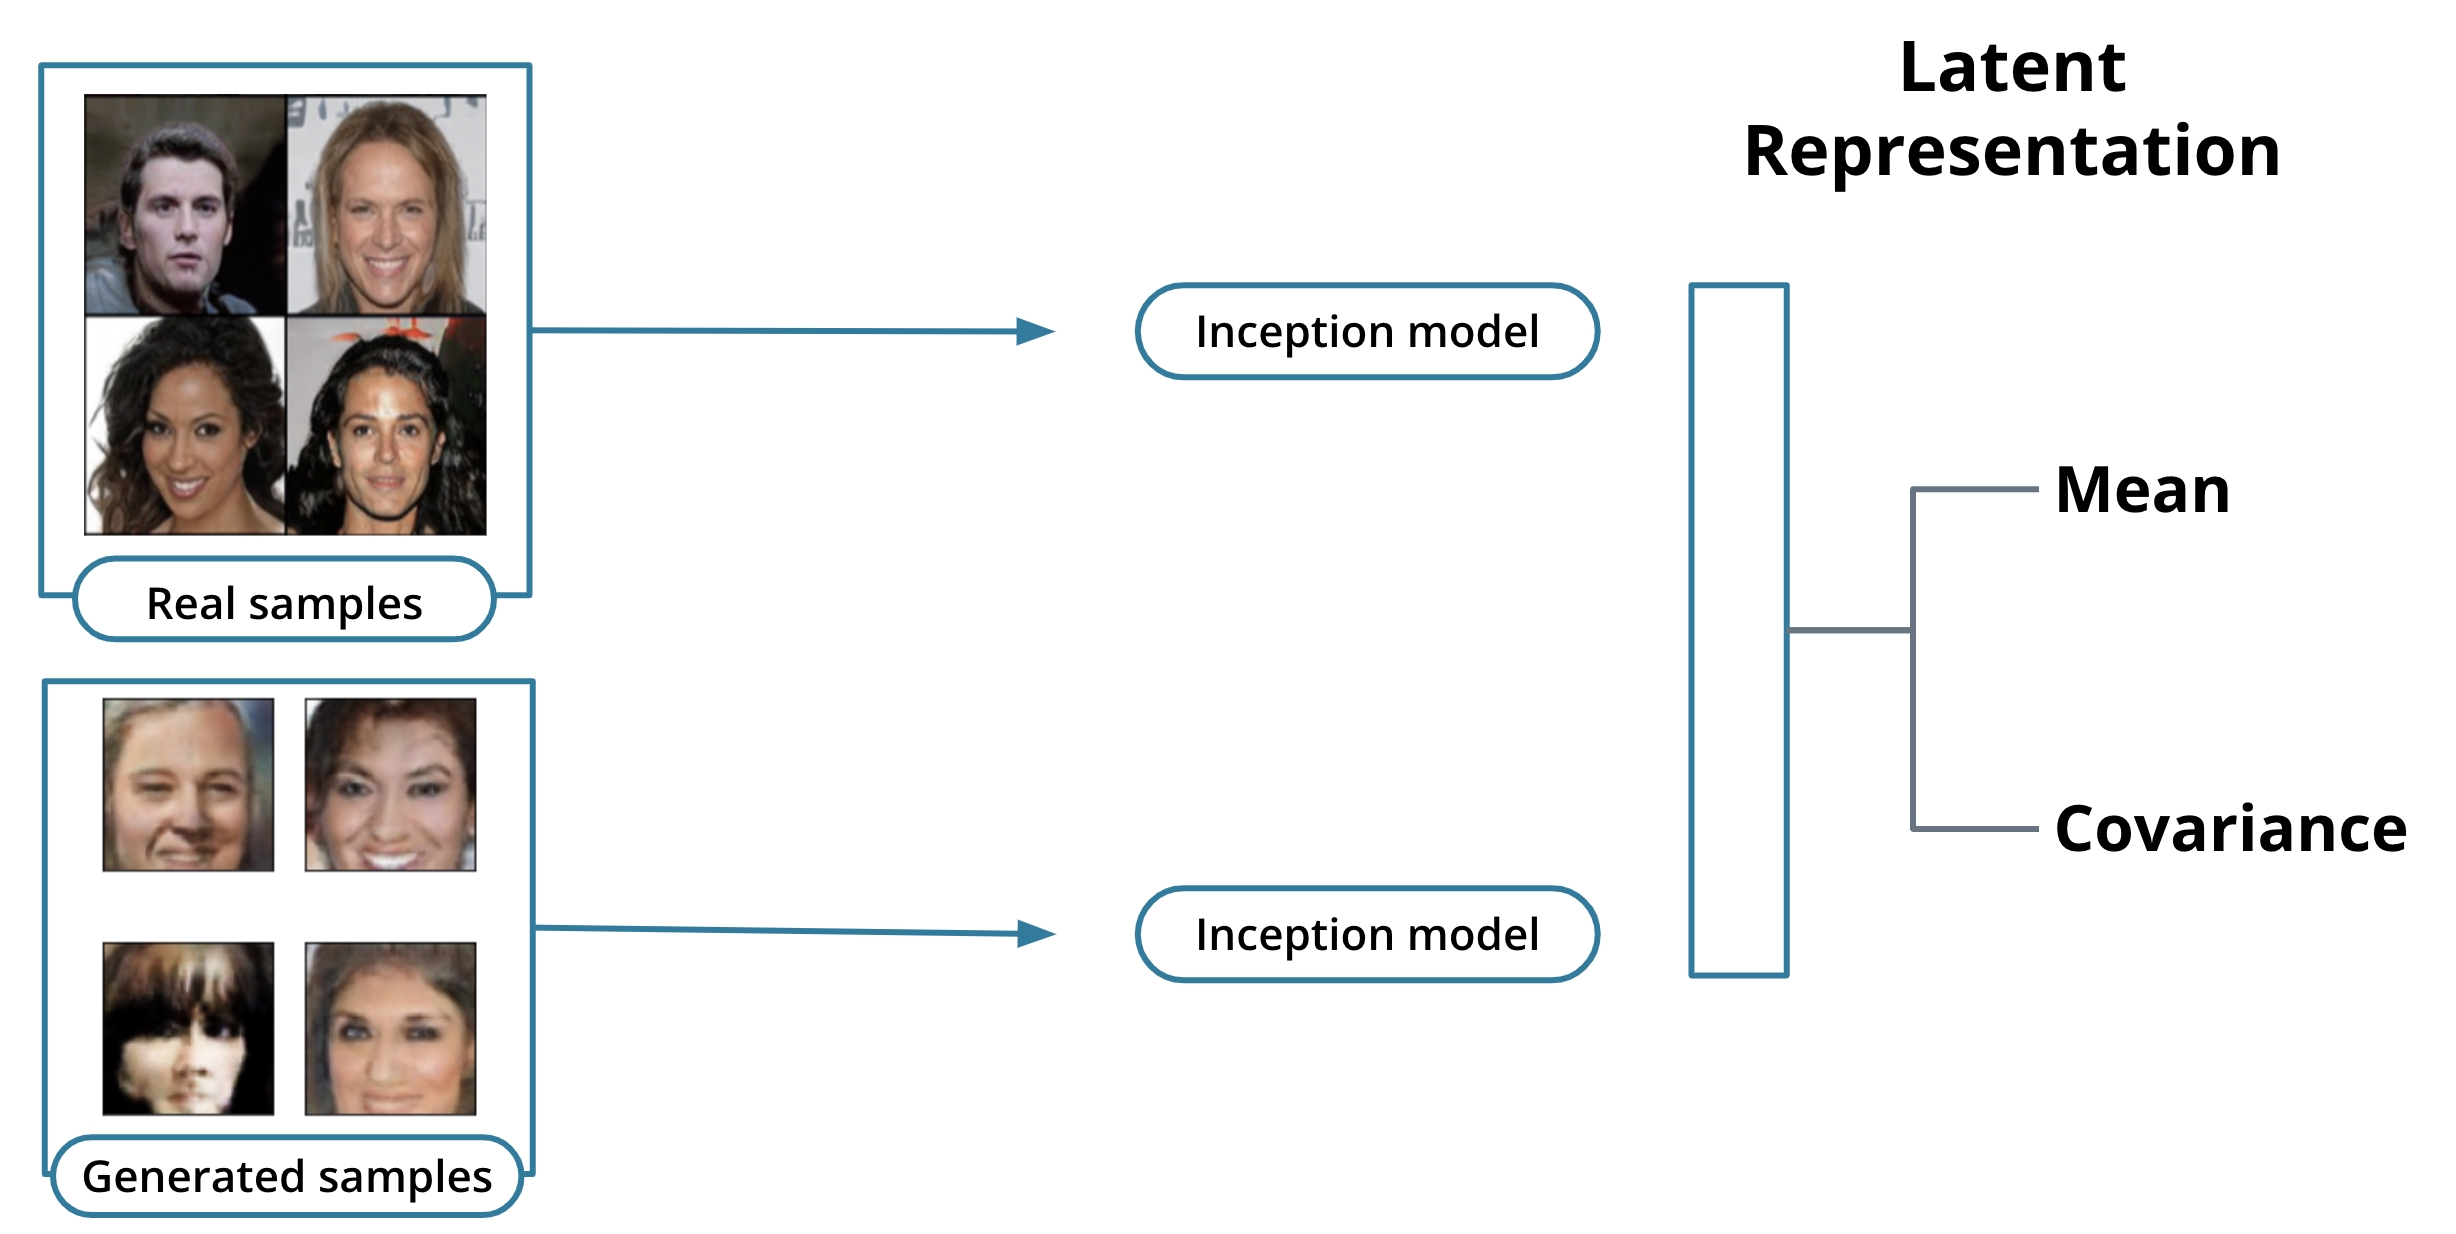
\includegraphics[width=0.75\linewidth]{img//genAdvNet//deepGAN/screen-shot-2022-05-11-at-4.30.32-pm.jpeg}
The mathematical equation for determining FID is: \[d = ||m_r - m_f||_{2}^{2} + Tr(C_r + C_f -2(C_r C_f)^{(1/2)})\]
where
\begin{itemize}
    \item \(m_r\): mean of the real distribution
    \item \(C_r\): covariance of the real distribution
    \item \(m_f\): mean of the fake distribution
    \item \(C_f\): covariance of the fake distribution
    \item \(T_r\): trace
\end{itemize}
The \href{https://arxiv.org/pdf/1606.03498.pdf}{\textbf{Inception Score paper}} and the \href{https://arxiv.org/pdf/1706.08500.pdf}{\textbf{Frechet Inception Distance paper}} (which is also the TTUR paper, suprise!) contain a lot more information about the implementation of both metrics. \newline

Both official implementations are available:
\begin{itemize}
    \item \href{https://github.com/openai/improved-gan}{\textbf{Inception Score Code}}
    \item \href{https://github.com/bioinf-jku/TTUR}{\textbf{Frechet Inception Distance code}}
\end{itemize}
I encourage you to take a look at the code as you will have to implement both of these metrics in the next exercise.

\subsection{Quiz Question}

Which of the following statement are true? (Check all that apply)
\begin{itemize}
    \item \textbf{The inception score only requires generated images.}
    \item \textbf{The inception score requires to calculate the KL divergence between the conditional label distribution and the marginal distribution.}
    \item \textbf{The Frechet Inception Distance requires both the mean and covariance of the generated samples and the real samples.}
    \item \textbf{The Frechet Inception Distance calculates the distance between two multivariate Gaussian distributions}
\end{itemize}

Solution: FID and IS are both metrics to evaluate GANs. The IS only uses the generated images whereas the FID requires statistics over both the generated and real dataset.

\section{Exercise Part 3: IS FID}
\subsection{Inception Score (IS) and Frechet Inception Distance
(FID)}

Both the Inception Score (or IS) and the Frechet Inception Distance (or
FID) are metrics to assess the quality of images generated by a GAN.

\subsubsection{Generated data}

To calculate the Inception Score and the Frechet Inception Distance, we
are going to use some generated samples from the previous exercise. The
\lstinline{samples.pickle} contains 800 samples recorded
over 50 epochs (16 samples per epoch). We can visualize them below. The
samples are saved as \lstinline{np.array} and contain
images in the {[}0, 255{]} range.

\begin{lstlisting}[language=Python]
# run this cell once to install the dependency
# you will have to restart the kernel afterwards
!pip install ipywidgets
\end{lstlisting}

\begin{lstlisting}[language=Python]
import pickle
from typing import List

import matplotlib.pyplot as plt
import numpy as np
\end{lstlisting}

\begin{lstlisting}[language=Python]
# helper function for visualization.

def view_samples(epoch: int, samples: List[np.array]):
    fig, axes = plt.subplots(figsize=(14,4), nrows=2, ncols=8, sharey=True, sharex=True)
    for ax, img in zip(axes.flatten(), samples[16 * epoch: 16 * (epoch + 1)]):
        ax.xaxis.set_visible(False)
        ax.yaxis.set_visible(False)
        im = ax.imshow(img.reshape((32,32,3)))
    plt.show()
\end{lstlisting}

\begin{lstlisting}[language=Python]
with open('../samples.pkl', 'rb') as f:
    samples = pickle.load(f)
\end{lstlisting}

\begin{lstlisting}[language=Python]
view_samples(49, samples)
\end{lstlisting}

\subsubsection{Inception score}

The Inception Score was introduced by the
\href{https://arxiv.org/pdf/1606.03498.pdf}{Improved Techniques for
Training GANs} paper. This metric relies on the following approach: 
\begin{itemize}
    \item generated images are fed through the \href{https://arxiv.org/pdf/1409.4842.pdf}{Inception model} pretrained on the ImageNet dataset
    \item the probability distribution for each image should have \href{https://en.wikipedia.org/wiki/Entropy_(information_theory)}{low-entropy}. In other words, the model should output high probabilities for a single class and be confident that the image contains one object. We call this distribution the \textbf{conditional label distribution}.
    \item the probability distribution of all the classes over the whole dataset should have high entropy, meaning that the generative model creates images with high variability. We call this distribution the \textbf{marginal distribution}.
\end{itemize}
The inception score is calculated using the
\href{https://en.wikipedia.org/wiki/Kullback\%E2\%80\%93Leibler_divergence}{Kullback--Leibler
Divergence} (KL Divergence).

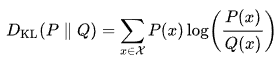
\includegraphics[width=1\linewidth]{img//genAdvNet//deepGAN/kl_divergence.png}

The KL divergence is a measure of how two distributions are similar.
Since we want the conditional label distribution to have
\href{https://en.wikipedia.org/wiki/Entropy_(information_theory)}{low
entropy} (think of a very low spread gaussian for example) and the
marginal distribution to have high entropy (think uniform distribution),
we want to \textbf{maximize the KL divergence}.

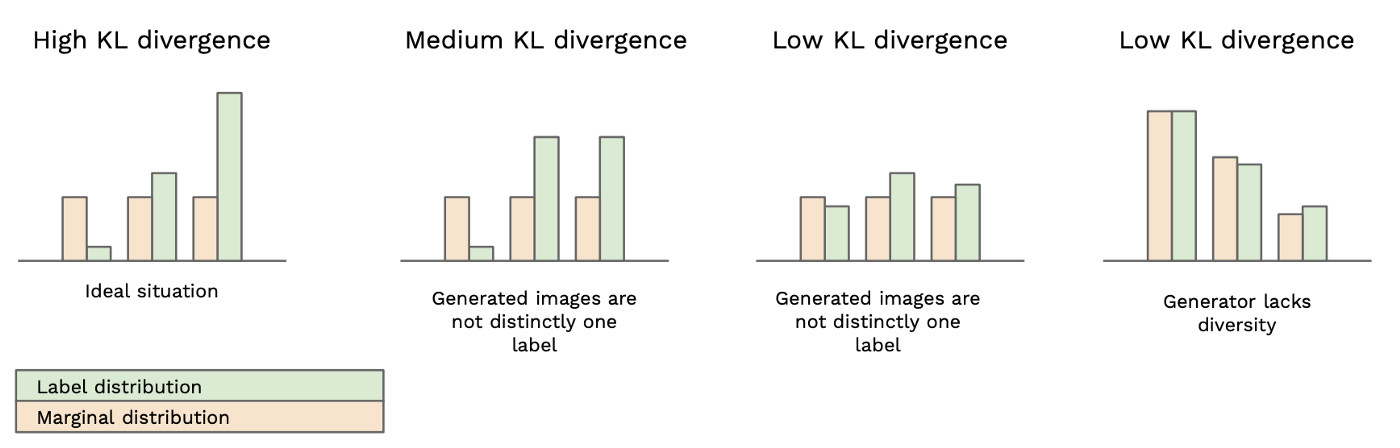
\includegraphics[width=1\linewidth]{img//genAdvNet//deepGAN/fid_score.png}

\href{https://medium.com/octavian-ai/a-simple-explanation-of-the-inception-score-372dff6a8c7a}{This article} explains the inception score in great depth.

\paragraph{Tips:}

\begin{itemize}
\item the \lstinline{inception_v3} pytorch model outputs the logits, not the probability and you will need to use the softmax activation to get probabilities.
\item look at the \href{https://docs.scipy.org/doc/scipy/reference/generated/scipy.stats.entropy.html}{scipy.stats.entropy}
  function for the kl divergence calculation.
\item you can find the pytorch Inception\_v3 model \href{https://pytorch.org/hub/pytorch_vision_inception_v3/}{here}. Don't forget to reshape the inputs!
\item if you are stuck, you can find the pytorch implementation of the inception score from the authors of the paper \href{https://github.com/openai/improved-gan/blob/master/inception_score/model.py}{here}.
\end{itemize}

\paragraph{Notes:}
In the original paper, they recommend to use 10 splits and calculate the mean and standard deviation of the score over the 10 splits. They also recommend to use large datasets (over 50k images). Here, we are using a small dataset and therefore will not take the split approach.

\begin{lstlisting}[language=Python]
import torch
from PIL import Image
from torchvision import transforms
from torchvision.models.inception import inception_v3
from scipy.stats import entropy
\end{lstlisting}

\begin{lstlisting}[language=Python]
def calculate_scores(samples: List[np.ndarray]) -> List[np.ndarray]:
    """
    This function calculates the score for each sample.
    """
    # load model
    inception_model = inception_v3(pretrained=True, transform_input=False)
    inception_model.eval()
    inception_model.cuda()
    
    # preprocessing
    preprocess = transforms.Compose([
        transforms.Resize(299),
        transforms.CenterCrop(299),
        transforms.ToTensor(),
        transforms.Normalize(mean=[0.485, 0.456, 0.406], std=[0.229, 0.224, 0.225]),
    ])    
    
    # forward pass
    scores = []
    for image in samples:
        image = Image.fromarray(image)
        input_tensor = preprocess(image)
        input_batch = input_tensor.unsqueeze(0).cuda()
        output = inception_model(input_batch)
        probs = torch.nn.functional.softmax(output[0].cpu().detach(), dim=0)
        scores.append(probs.numpy())
    return scores
\end{lstlisting}

\begin{lstlisting}[language=Python]
scores = calculate_scores(samples)
\end{lstlisting}

\begin{lstlisting}[language=Python]
def get_inception_score(scores: List[np.ndarray]) -> float:
    total_scores = []
    py = np.mean(scores, axis=0)

    # calculate the kl divergence
    kl = []
    for pyx in scores:
        ent = entropy(pyx, py)
        kl.append(ent)
    return np.exp(np.mean(kl))
\end{lstlisting}

\begin{lstlisting}[language=Python]
inception_score = get_inception_score(scores)
print(inception_score)
\end{lstlisting}

\subsubsection{Frechet Inception Distance}

The Frechet Inception Distance was first introduced by the
\href{https://arxiv.org/pdf/1706.08500.pdf}{GANs Trained by a Two
Time-Scale Update Rule Converge to a Local Nash Equilibrium} paper. \newline

The Inception Score was a groundbreaking metric for measure GAN
performances but it has a major flaw: \textbf{it does not take into
account the statistics of the ``real'' dataset the GAN is supposed to
mimic and only uses the generated images.} \newline

The FID takes a different approach: 
\begin{itemize}
    \item for each image in the generated dataset \textbf{and} the target (real) dataset, get the latent representation by running the Inception model. The latent representation of each image is the output of the penultimate layer, before the final classification layer.
    \item calculate the mean and the covariance of the real distribution (\(m_{r}\) and \(C_{r}\))
    \item calculate the mean and the covariance of the generated distribution (\(m_{g}\) and \(C_{g}\))
    \item calculate the Frechet Distance defined below:
\end{itemize}

\(FID = ||m_{r} - m_{g}||^{2}_{2} + Tr(C_{r}) + Tr(C_{g}) - 2 Tr(C_{r}C_{g})^{1/2}\)

where \(||.||_{2}\) is the L-2 norm and \(Tr\) the trace of the
covariance matrices. \newline

In this exercise, we will simply ask you to implement the FID
calculation, assuming that you already have calculated the mean and
covariance of both distribution.

\paragraph{Tips:}
\begin{itemize}
\item you can calculate the trace of the covariance matrices using \lstinline{np.trace}
\end{itemize}

\begin{lstlisting}[language=Python]
from scipy import linalg
\end{lstlisting}

\begin{lstlisting}[language=Python]
def get_fid(mu1: np.array, sigma1: np.array, mu2: np.array, sigma2: np.array):
    """
    Calculate the FID. 
    """
    diff = mu1 - mu2
    
    # calculate the square root of the dot product of the covariance matrices
    covmean, _ = linalg.sqrtm(sigma1.dot(sigma2), disp=False)
    
    # calculate the trace
    tr_covmean = np.trace(covmean)

    return (diff.dot(diff) + np.trace(sigma1)
            + np.trace(sigma2) - 2 * tr_covmean)
\end{lstlisting}

\begin{lstlisting}[language=Python]
samples1 = np.random.randn(100, 2048)
mu1 = np.mean(samples1, axis=0)
sigma1 = np.cov(samples1)

samples2 = np.random.randn(100, 2048)
mu2 = np.mean(samples2, axis=0)
sigma2 = np.cov(samples2)
\end{lstlisting}

\begin{lstlisting}[language=Python]
fid = get_fid(mu1, sigma1, mu2, sigma2)
print(fid)
\end{lstlisting}


Solution on \href{https://www.youtube.com/watch?v=UBrNxK0Gkao&t=2s}{Youtube}

\section{Other Applications of GANs}
So far, you've seen a lot of examples of how GANs might be used for image generation and transformation. GANs are a relatively new formulation and so there are some really exciting research directions that include GANs. I didn't have time to cover them all in video, so I wanted to highlight a few of my favorite examples, here, and link to some resources that I've found helpful! \textbf{This page is for those who are interested in learning more about GANs and curious to learn about semi-supervised learning.}

\subsection{Semi-Supervised Learning}

Semi-supervised models are used when you only have a \textit{few} labeled data points. The motivation for this kind of model is that, we increasingly have a lot of raw data, and the task of labelling data is tedious, time-consuming, and often, sensitive to human error. Semi-supervised models give us a way to learn from a large set of data with only a few labels, and they perform surprisingly well even though the amount of labeled data you have is relatively tiny. Ian Goodfellow has put together a video on this top, which you can see, below. \newline

\href{https://www.youtube.com/watch?v=_LRpHPxZaX0}{Youtube}
\subsubsection{Semi-Supervised Learning in PyTorch}
There is a readable implementation of a semi-supervised GAN from the repository \href{https://github.com/Sleepychord/ImprovedGAN-pytorch}{\textbf{Improved GAN (Semi-supervised GAN)}}. If you'd like to implement this in code, I suggest reading through that code!

\subsubsection{Domain Invariance}
Consider \href{https://arxiv.org/abs/1709.02480}{\textbf{the car classification example from the research paper on arXiv}}. From the abstract, researchers (Timnit Gebru, et. al) wanted to:

\begin{quote}
develop a computer vision pipeline to predict income, per capita carbon emission, crime rates and other city attributes from a single source of publicly available visual data. We first detect cars in 50 million images across 200 of the largest US cities and train a model to predict demographic attributes using the detected cars. To facilitate our work, we have collected the largest and most challenging fine-grained dataset reported to date consisting of over 2600 classes of cars comprised of images from Google Street View and other web sources, classified by car experts to account for even the most subtle of visual differences.

\end{quote}

One interesting thing to note is that these researchers obtained some manually-labeled Streetview data \textit{and} data from other sources. I'll call these image sources, domains. So Streetview is a domain and another source, say cars.com is separate domain.

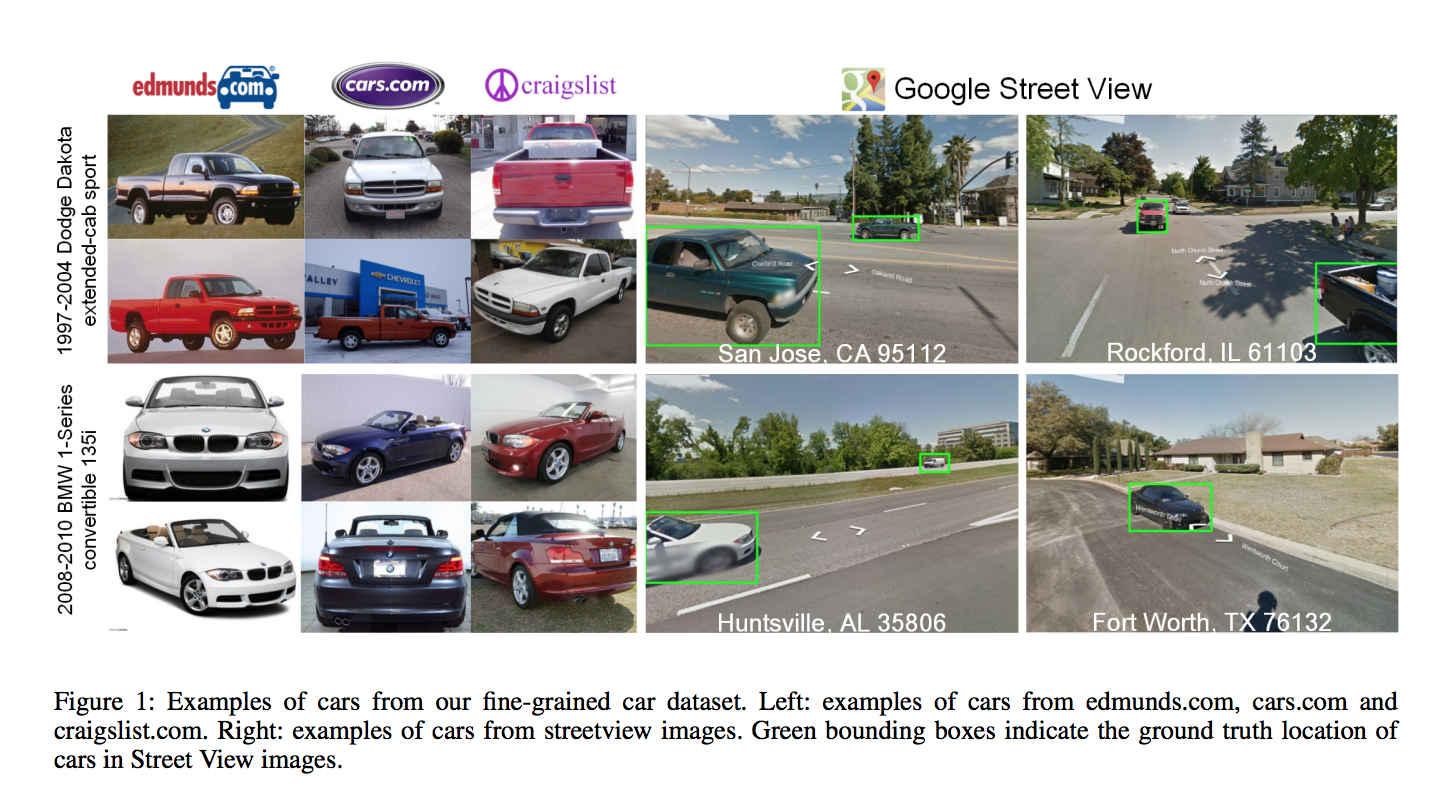
\includegraphics[width=1\linewidth]{img//genAdvNet//deepGAN/screen-shot-2018-11-13-at-3.06.36-pm.png}
\captionof{figure}{Images from the paper, Fine-Grained Car Detection for Visual Census Estimation}

The researchers then had to find a way to combine what they learned from these multiple sources! They did this with the use of multiple classifiers; adversarial networks that do \textit{not} include a Generator, just two classifiers.

\begin{quote}

\begin{itemize}
    \item One classifier is learning to recognize car types
    \item And another is learning to classify whether a car image came from Google Streetview or cars.com, given the extracted features from that image
\end{itemize}

\end{quote}

So, the first classier’s job is to classify the car image correctly \textit{and} to \textbf{trick the second classifier} so that the second classifier cannot tell whether the extracted image features indicate an image from the Streetview or cars.com domain! \newline

The idea is: if the second classifier cannot tell which domain the features are from, then this indicates that these features are shared among the two domains, and you’ve found features that are \textbf{domain-invariant}. \newline

Domain-invariance can be applied to a number of applications in which you want to find features that are invariant between two different domains. These can be image domains or domains based on different population demographics and so on. This is also sometimes referred to as \href{https://arxiv.org/pdf/1705.11122.pdf}{\textbf{adversarial feature learning}}.
\subsection{Ethical and Artistic Applications: Further Reading}
\begin{itemize}
    \item \href{https://www.newyorker.com/magazine/2018/11/12/in-the-age-of-ai-is-seeing-still-believing}{\textbf{Ethical implications of GANs}} and when "fake" images can give us information about reality.
    \item \href{https://www.ssense.com/en-us/editorial/fashion/do-androids-dream-of-balenciaga-ss29}{\textbf{Do Androids Dream in Balenciaga?}} note that the author briefly talks about generative models having artistic potential rather than ethical implications, but the two go hand in hand. The generator, in this case, will recreate what it sees on the fashion runway; typically thin, white bodies that do not represent the diversity of people in the world (or even the diversity of people who buy Balenciaga).
\end{itemize}

\subsection{GANs for Illuminating Model Weaknesses}
GANs are not only used for image generation, they are also used to find weaknesses in existing, trained models. The adversarial examples that a generator learns to make, can be designed to \textit{trick} a pre-trained model. Essentially, small perturbations in images can cause a classifier (like AlexNet or a known image classifier) to fail pretty spectacularly!

\begin{quote}
\href{https://openai.com/index/attacking-machine-learning-with-adversarial-examples}{\textbf{The OpenAI blog post: Attacking machine learning with adversarial examples}} details how adversarial examples can be used to "attack" existing models, and discusses potential security issues. And one example of a perturbation that causes misclassification can be seen below.

\end{quote}

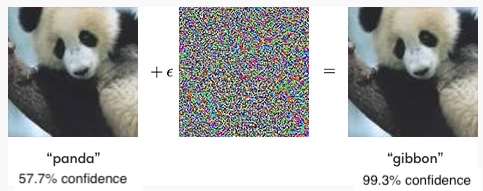
\includegraphics[width=0.75\linewidth]{img//genAdvNet//deepGAN/openai-attacking-machine-learning-with-adversarial-examples.jpeg}
\captionof{figure}{Image of a panda misclassified as an ape}

Adding a small amount of noise to an image of a panda causes a model to misclassify it as a \href{https://en.wikipedia.org/wiki/Gibbon}{\textbf{gibbon}}, which is a kind of ape. One of the interesting parts of this is the model's confidence. With this noise it is \textbf{99.3}\% confident that this is an image of a gibbon, when we can pretty clearly see that it is a panda!

\section{Lesson Review}
\href{https://www.youtube.com/watch?v=84LLLNYDrRM}{Youtube} \newline

In this lesson you:

\begin{itemize}
    \item Built a DCGAN model using convolution, transpose convolution and batch normalization layers to build the generator and the discriminator models
    \item Trained a DCGAN model on the CIFAR10 dataset and discovered the importance of hyperparameters
    \item Implemented two metrics to evaluate GAN performances and generated samples
\end{itemize}
You now have the tools to build GANs on more complex datasets.
